% =====================================================================
% paper06_assessment_separation_v77
% Parent: Paper06 v76 (preserved unchanged); local-only audit-repair derivative.
% v77 (2026-10-27): substantive claim, unit, verification, benchmark and reference repairs.
% No external release or deposit is authorized by this revision.
% Build: tectonic paper06_assessment_separation_v77.tex (elsarticle, authoryear)
% =====================================================================
\documentclass[preprint,11pt,authoryear]{elsarticle}

\usepackage{amsmath,amssymb,amsthm}
\usepackage{booktabs}
\usepackage{array}
\usepackage{tabularx}
\usepackage{graphicx}
\graphicspath{{./}{figs/}{paper06_assessment_separation_v77_src/figs/}}
\usepackage{enumitem}
\usepackage[colorlinks=true,urlcolor=blue,linkcolor=blue,citecolor=blue]{hyperref}
\emergencystretch=3em
\setlength{\tolerance}{2000}

\newtheorem{theorem}{Theorem}
\newtheorem{proposition}{Proposition}
\newtheorem{lemma}{Lemma}
\newtheorem{corollary}{Corollary}
\theoremstyle{definition}
\newtheorem{definition}{Definition}
\theoremstyle{remark}
\newtheorem{remark}{Remark}

\newcommand{\Etyp}{E_{\mathrm{typ}}}
\newcommand{\Eend}{E_{\mathrm{end}}}
\newcommand{\Ephys}{E_{\mathrm{tube,phys}}}
\newcommand{\Vtyp}{\mathcal{V}_{\mathrm{typ}}}
\newcommand{\Vweak}{\mathcal{V}_{\mathrm{weak}}}
\newcommand{\Vphys}{\mathcal{V}_{\mathrm{phys}}}
\newcommand{\Vend}{\mathcal{V}_{\mathrm{end}}}
\newcommand{\Wp}{W_+}
\newcommand{\FP}{\mathrm{FP}_{\mathrm{agg}}}
\newcommand{\Tube}{\mathrm{Tube}}
\newcommand{\Succ}{\mathrm{Succ}}
\newcommand{\End}{\mathrm{End}}
\newcommand{\conv}{\operatorname{conv}}
\newcommand{\Rp}{\mathbb{R}^n_+}
\newcommand{\Q}{\mathcal{Q}}
\newcommand{\act}[1]{\textsc{#1}}

\journal{Journal of Multi-Criteria Decision Analysis}

\begin{document}

\begin{frontmatter}

\title{Transition Certification with Composite Indices: The Acceptance Gap Between Compensatory and Noncompensatory Rules}

\author[1]{Amin Abaee\corref{cor1}}
\ead{amin_abaee@ut.ac.ir}
\cortext[cor1]{Corresponding author. ORCID: 0000-0002-0019-1842.}
\affiliation[1]{organization={Independent Researcher}, city={Tehran}, country={Iran}}

\begin{abstract}
Composite indices can certify transitions under weight-adaptive or common-plan rules. We formulate the comparison as a robust finite-horizon assessment with path-wise constraints and declared disturbances. The full-cone aggregate is lossless at a fixed trajectory, yet the plan/weight quantifiers need not commute. For finite menus in the stated margin-first class, the weight-adaptive accepted set is $\conv(\mathcal D)+\Rp$ and the common-plan set is the union of single-plan acceptance orthants; an abstract convexification of required margins closes that gap, while physical implementation requires a separate control assumption.

An exact rational witness has a nonempty gap interior: at its canonical point both normalized margins are $6/5$, so the equal-weight margin sum $s_1+s_2=12/5$ exceeds the witness's licensing threshold $2$; each weighting licenses at least one primitive plan, though no single primitive plan meets both typed floors. A closed-form reserve threshold separates rescuable from impossible states. Under the declared linear-flow blend, fractional control closes the action-indexed gap, while the specified shared-shock blend does not restore feasibility at the canonical point; the complete-excursion result is conditional on its union-of-tubes assumption. On the witness-defined diagonal slice, every positive-elasticity member of the stated CES family falsely certifies an exact interval; the Leontief limit is typed-safe under the declared collapse convention. The shared-shock gap survives the exact $1/2$-cut, while a distinct replace reading with identical plan- and weight-independent dips collapses the distinction (SI S4). Northern-cod values supply a historical unit comparison only; the benchmark is not a fitted fishery model.
\end{abstract}

\begin{keyword}
multi-criteria decision analysis \sep compensatory and noncompensatory aggregation \sep composite indicators \sep scalarization \sep robustness \sep sustainability assessment \sep viability
\end{keyword}

\end{frontmatter}

\section{Introduction}\label{sec:intro}

\subsection{Compensability as an acceptance question}

Whenever decision-makers assess a sustainability transition, they face a familiar question: can strength in one area make up for failure in another? Multi-attribute value theory builds trade-offs into its value structure \citep{KeeneyRaiffa1976}. Outranking methods, by contrast, limit compensation through concordance and veto conditions \citep{Roy1996,Vincke1992}; work on sustainable development has also emphasized the incommensurability of some criteria \citep{Munda2005,MartinezAlier1998}.

The same question appears in environmental assessment as the distinction between weak and strong sustainability. \emph{Weak sustainability} represents substitution among forms of capital through an aggregate that must not decline \citep{WorldBank2011,Neumayer2013,Boos2015}. \emph{Strong sustainability} treats selected stocks as separately binding \citep{Daly1990,Ekins2003}. Research on the indicator theory of these positions is well developed, as is the analysis of compensability in the multi-criteria methods used for sustainability assessment \citep{Hanley1999,Martinet2011,CairnsMartinet2014,DoyenGajardo2020,Usubiaga2025,Cinelli2014,Schar2025}.

Much of this work classifies aggregation at a fixed profile of criterion values—a snapshot. This paper asks a different question, about \emph{transitions}: when a plan unfolds over time under declared disturbances, and several criteria must hold along the entire path, when can a compensatory aggregate certify a transition that a noncompensatory assessment rejects? The question is not how weights should be chosen; methods for eliciting them are well developed \citep{Nardo2008,Becker2017}. Nor is it the familiar static limitation of weighted sums in recovering nonconvex parts of a Pareto front \citep{DasDennis1997}. The focus is \emph{acceptance semantics}: the rule that classifies a composite reading of a transition as accepted or rejected—the sorting problem of decision aiding \citep{Roy1996}.

\subsection{Two acceptance semantics}

To see where the two assessments can diverge, imagine the transition problem at state $z$. It tracks typed-margin coordinates $s_i$, each expressed after a declared positive reference scale has been chosen so that zero is its binding floor, and has a finite menu $\mathcal A$ of plans and a declared disturbance set $D$. The weights act on these normalized coordinates; they do not turn unlike physical quantities into a conservation law. Both assessments impose the same physical safe and destination sets $S^{\mathrm{phys}}$ and $G^{\mathrm{phys}}$. Exact-tube semantics checks the entire path, not just its endpoint: for every $d\in D$, a plan's full tube must remain in $S^{\mathrm{phys}}$, and its successor set must lie in $G^{\mathrm{phys}}$.

\begin{samepage}
Now consider the floor test. Write $s(p)=(s_1(p),\dots,s_n(p))$ for the typed-margin vector at state $p$. For each weight $w$ in the full nonnegative cone $\Wp=\Rp\setminus\{0\}$, let $E_w(z)$ be the menu plans that meet those shared requirements and also keep $w\cdot s(p)\ge0$ at every tube state and every successor state, for every $d\in D$. Let $\Etyp(z)$ be the menu plans that meet the same physical, destination, and disturbance requirements but keep each typed floor $s_i(p)\ge0$ at those same states. Thus the two assessments share physical feasibility, destination attainment, and disturbance coverage; only the test applied to the typed margins differs.
\end{samepage}

The key choice is simple: must one plan work for every weighting, or may each weighting have its own plan? Formally, the two acceptance rules differ only in the order of the quantifiers:
\begin{itemize}[leftmargin=2em]
\item \emph{Common-plan acceptance}: $\exists a\in\mathcal A\;\forall w\in\Wp:\ a\in E_w(z)$. One plan must work for every weighting.
\item \emph{Weight-adaptive acceptance}: $\forall w\in\Wp\;\exists a_w\in\mathcal A:\ a_w\in E_w(z)$. For each weighting, some plan works; it may be a different one.
\end{itemize}
The first rule implies the second, but the converse need not hold. Because $\Wp$ contains every coordinate weight, the full-cone identity is $\Etyp(z)=\bigcap_{w\in\Wp}E_w(z)$. Among plans meeting the shared requirements, a single plan passes every weight exactly when it satisfies each typed floor; equivalently, common-plan acceptance is $\exists a\in\Etyp(z)$. The gap, when it occurs, comes from the weight-adaptive rule's ability to use different plans for different weights. This quantifier gap can occur even for static alternative margin vectors; here the tubes and disturbances supply its transition-assessment setting. Table~\ref{tab:protocols} places these two rules among the four protocols considered in the paper.

\begin{table}[!htbp]
\centering\small
\caption{Four acceptance protocols for a composite index on a transition datum. Protocols 3 (common-plan robustness) and 4 (typed acceptance) have the same accepted-plan and accepted-state sets on the full cone (Proposition~\ref{prop:hierarchy}(ii)); they are shown separately to distinguish the common-plan and typed formulations. The separation is Protocol 2 against either equivalent form.}
\label{tab:protocols}
\begin{tabularx}{\textwidth}{>{\raggedright\arraybackslash}p{0.25\textwidth} >{\raggedright\arraybackslash}p{0.27\textwidth} X}
\toprule
Protocol & Quantifier form & Reading \\
\midrule
1. Fixed-weight assessment & $a\in E_w(z)$ at a declared $w$ & one index, one selected plan: ordinary fixed-weight certification \\
2. Weight-adaptive (per-weight) acceptance & $\forall w\ \exists a_w\in E_w(z)$ & for each weighting $w$, some plan $a_w$ is licensed; the plan may vary with $w$: the compensatory reading, $\Vweak=\bigcap_w\mathcal V_w$ \\
3. Common-plan robustness & $\exists a\ \forall w:\ a\in E_w(z)$ & one plan serves every weighting; equivalent to Protocol 4 on the full cone \\
4. Coordinate-wise (typed) acceptance & $\exists a:\ a\in\Etyp(z)$ & separately binding floors enforced path-wise; equivalent to Protocol 3 on the full cone \\
\bottomrule
\end{tabularx}
\end{table}

An analogous split appears in adjustable robust optimisation: a here-and-now decision is fixed before the relevant parameter is known, while a wait-and-see decision may depend on it. Here the assessment weight plays the role of that parameter \citep{BenTal2004}. This is an analogy for the order of the acceptance rule, not a claim about how real auditors or policymakers behave. The result concerns a certification protocol applied to a composite index, not the suitability of composite indices as descriptive summaries.

The witness makes the split concrete. \act{fast} risks the first floor, \act{slow} the second. \act{staged} protects both only when the reserve covers its bridge; \act{no-switch} misses the destination. At the action-indexed canonical point $(x,s_1,s_2)=(\tfrac12,\tfrac65,\tfrac65)$, $s_1+s_2=\tfrac{12}5\ge2$, so every $w\in\Wp$ licenses \act{fast} or \act{slow}, yet none of the four plans is typed-admissible. This verdict is specific to the stated menu and disturbance class.


\pagebreak
\subsection{Contributions}

The paper makes five contributions, stated in the order of the text.
\begin{enumerate}[leftmargin=2em,label=(\roman*)]
\item \emph{Localisation and hierarchy} (Section~\ref{sec:general}). On the full cone the typed operator is exactly the common-plan intersection, $\Etyp(z)=\bigcap_{w\in\Wp}E_w(z)$, and at any fixed trajectory the aggregate is lossless (Lemma~\ref{lem:cone}); the chain typed $\subseteq$ scalarized $\subseteq$ physical $\subseteq$ endpoint holds for every weight, and restricting a nonempty weight family can only enlarge the compensatory accepted set (Propositions~\ref{prop:hierarchy}--\ref{prop:monotone}). The quantifier separation itself is a plan-selection phenomenon and can occur for static alternatives; the finite-horizon paths specify how the margins are generated in the transition application.
\item \emph{A finite-menu geometric characterisation} (Theorem~\ref{thm:menu}). Under the explicit margin-first hypothesis $m_a(w)=w\cdot d_a$, weight-adaptive acceptance is $\conv(\mathcal D)+\Rp$ and common-plan acceptance is $\bigcup_a(d_a+\Rp)$. Convexifying required-margin vectors closes this abstract gap; physical convexification of controls is a separate implementability assumption. Lemma~\ref{lem:sync} identifies when the margin-first path requirement agrees exactly with scalarizing after the within-path maximum.
\item \emph{An explicit rational witness} (Theorem~\ref{thm:witness}). On a four-plan datum the gap is a region with nonempty interior, equal to the \emph{impossibility region} $I$; the aggregate-versus-floor discrepancy region splits at the reserve level $x=1$ into $I$ and a \emph{rescue set} $R$ that a reserve-financed staged plan already serves; exact thresholds $\rho_1=(2-s_1)/s_2$ and $\rho_2=s_1/(2-s_2)$ locate the licensing regions of the two principal plans, with coordinate-axis weights classified separately; and the minimal reserve increment that converts impossibility into rescue is $\kappa^*(z)=(1-x)\,\mathbf 1[z\notin\Vtyp]$ (Proposition~\ref{prop:rescue}). The separation persists under hold-prefix extension of the horizon; a separate two-stage construction shows one way a repair stage can erase it by enlarging the next-stage accepted sets while retaining the same final terminal rules (Proposition~\ref{prop:persist}). The quantifier gap is sufficient but not necessary for false acceptance: at the canonical point $(x,s_1,s_2)=(1/2,6/5,6/5)$ the single fixed weight $(1,1)$ already accepts a primitive plan, because $12/5\ge2$, while no primitive plan meets both typed floors (Remark~\ref{rem:fixedweight}).
\item \emph{What closes the gap and what does not} (Theorem~\ref{thm:blend}, Proposition~\ref{prop:timeshare}). Fractional blending of the primitive plans -- menu convexification at the level of control flows -- makes the typed accepted set of the action-indexed margin class coincide exactly with the compensatory region, so that gap is a property of the finite deterministic menu, not of either doctrine. The statement is class-specific: under the shared-shock class the blend window is empty at the canonical point ($12/5<5/2$), so blending does not close that gap (Proposition~\ref{prop:commonshock}). The complete-excursion result is conditional on a policy whose visited set is the union of both full primitive tubes; it does not characterize ordinary finite-rate switching. A distinct three-switch implementation keeps both canonical margins positive, so no general failure of finite switching is claimed.
\item \emph{Robustness of the separation to the aggregator and to the disturbance class} (Theorem~\ref{thm:ladder}, Proposition~\ref{prop:commonshock}). Replacing the linear index by a constant-elasticity-of-substitution (CES) aggregator with elasticity $\sigma$ changes the gap but does not remove it: the accepted rungs are nested, on the witness-defined diagonal gap slice, each positive-elasticity member falsely certifies an exact interval with critical floors $1<5/4<\sqrt2<\varphi<\sqrt3<\dots\to2$; therefore no positive elasticity is uniformly safe over the full gap, while the Leontief member ($\sigma=0$), which is the typed operator, is uniformly safe. Under a shared environmental shock striking every plan the gap survives, reduced by an exact $1/2$-cut, with the licensing thresholds unshifted on the surviving region; the reserve route then fails on an exact band of states.
\end{enumerate}
The analytic claims retained in the main text are proved in Appendices~\ref{app:general}--\ref{app:witness} and SI~S2--S4; finite-grid checks are supporting evidence, not continuum proofs. SI~S7 and Data Availability distinguish the checks that are present in versioned deposits from reported runs whose scripts or logs are not included. The pinned Lean source covers selected algebraic and finite-rung components, not the full continuum CES claims; its limits are summarized in SI~S7. Section~\ref{sec:benchmark} gives a synthetic Schaefer-style biomass illustration with an optional historical scale mapping, not an empirically calibrated fishery realization.

\paragraph{What is not claimed} No ranking of weak and strong sustainability as doctrines; no proof that any particular set of boundaries ought to be treated noncompensatorily; no empirical fit, forecast, validation, or performance result for a resource system (published DFO values are a limited scale/context anchor only); no infinite-horizon, stochastic or partially observed extension. The impossibility region is a negative certificate relative to the specified plan menu, and the separation is exhibited for a declared disturbance class.

\subsection{Position in the literature}

The backward constructions used here are typed instances of robust-predecessor, capture-basin and reach--avoid constructions \citep{Aubin1991,Aubin2011,SaintPierre1994,Lygeros1999,AubinCatte2002}; the hierarchy of Proposition~\ref{prop:hierarchy}(i) is constraint-set monotonicity of viability kernels \citep{Aubin1991,Frankowska1989}; viability methods are established in natural-resource management \citep{DeLaraDoyen2008,Doyen2012}. The plan/weight quantifier order is analogous to here-and-now versus wait-and-see decisions, but the assessment weight is not a realized disturbance and fractional physical control is not a randomization over plans. In composite-indicator practice the critique of weights as value judgements presented as measurement \citep{Hickel2020,Fischer2022} and the construction of indices without weights from Pareto fronts \citep{Gao2023} both concern the index; the result here concerns acceptance under a declared menu and rule. We do not assert priority over the elementary fact $\exists a\,\forall w\ne\forall w\,\exists a_w$, nor over the convex-hull geometry of multi-objective optimisation; Section~\ref{sec:related} states how those shared ingredients differ from the transition-certification question addressed here.

\section{Setting: typed transition data and assessment operators}\label{sec:setting}

\subsection{Typed transition data and exact-tube semantics}

A \emph{typed transition datum} consists of a state space $Z$ whose coordinates carry types (a conserved stock with a unit, a service margin, an institutional label), a finite \emph{menu} $\mathcal A$ of plans, a \emph{disturbance class} $D$, and, for each plan $a$ and disturbance $d$, a \emph{tube} $\Tube(a,d)\subseteq Z$ -- the full set of states visited during one review interval -- together with its \emph{endpoint set} $\End(a,d)\subseteq\Tube(a,d)$ and its \emph{successor set} $\Succ(a,d)$, the states reached after any end-of-interval reset. Among the coordinates are $n$ \emph{typed floors} $s=(s_1,\dots,s_n)$. Each raw margin $m_i$ is divided by a declared positive reference scale $q_i$, so $s_i=m_i/q_i$ is dimensionless and $s_i\ge0$ is the binding constraint; each floor retains its provenance (physical, contractual or normative). Typing records which quantities may be added: conservation statements are per type, and the framework does not itself authorize adding biomass, money and biodiversity into one conserved scalar. The weights act on these normalized coordinates as an assessment convention, not as a physical identity or automatic calibration.

Two constraint sets complete the datum: a \emph{physical safe set} $S^{\mathrm{phys}}$ and a \emph{physical destination set} $G^{\mathrm{phys}}$, which encode constraints that no assessment doctrine disputes (for instance that a reserve stock cannot be negative). The \emph{typed} sets add the floors,
\[
S=S^{\mathrm{phys}}\cap\{s_i\ge0,\ i=1,\dots,n\},\qquad G=G^{\mathrm{phys}}\cap\{s\ge0\},
\]
and the \emph{scalarized} sets at a weight $w$ add only the aggregate floor,
\[
S^w=S^{\mathrm{phys}}\cap\{w\cdot s\ge0\},\qquad G^w=G^{\mathrm{phys}}\cap\{w\cdot s\ge0\}.
\]
Throughout, $w$ ranges over the full nonnegative cone $\Wp=\Rp\setminus\{0\}$ unless a subfamily $W\subseteq\Wp$ is named. The semantics is \emph{exact-tube}: a plan is admissible only if every visited state, not merely the endpoint, lies in the relevant safe set. The disturbance quantifier is always innermost -- admissibility requires safety for every $d\in D$ -- and the separation studied here concerns a second quantifier, over weights, placed outside it.

\subsection{Assessment operators}

For a state $z$, four operators return the set of plans that an assessment doctrine accepts at $z$:
\begin{align}
\Etyp(z)&=\{a:\ \forall d\in D,\ \Tube(a,d)\subseteq S,\ \Succ(a,d)\subseteq G\}, \label{eq:Etyp}\\
E_w(z)&=\{a:\ \forall d\in D,\ \Tube(a,d)\subseteq S^w,\notag\\
&\qquad\Succ(a,d)\subseteq G^w\},\quad w\in\Wp, \label{eq:Ew}\\
\Ephys(z)&=\{a:\ \forall d\in D,\ \Tube(a,d)\subseteq S^{\mathrm{phys}},\notag\\
&\qquad\Succ(a,d)\subseteq G^{\mathrm{phys}}\}, \label{eq:Ephys}\\
\Eend(z)&=\{a:\ \forall d\in D,\ \End(a,d)\subseteq S^{\mathrm{phys}},\notag\\
&\qquad\Succ(a,d)\subseteq G^{\mathrm{phys}}\}. \label{eq:Eend}
\end{align}
$\Etyp$ is the \emph{noncompensatory typed} operator (each floor separately binding along the path); $E_w$ the \emph{scalarized} operator at weight $w$ (the dashboard reading $w\cdot s$ must stay nonnegative along the path); $\Ephys$ the \emph{physical} operator (no floors at all); and $\Eend$ the \emph{endpoint} operator, which represents any assessment architecture that evaluates constraints only at sampled or audited endpoints. The two axes along which they differ -- what is constrained and where it is evaluated -- are set out in Table~\ref{tab:semantics}; the typed-endpoint operator $E_{\mathrm{end,typ}}$, which applies the floors at endpoints only, is the remaining cell and is used once, in Section~\ref{sec:design}.

\begin{table}[!htbp]
\centering\small
\caption{Evaluation semantics: constraint structure (rows) by evaluation locus (columns).}
\label{tab:semantics}
\begin{tabularx}{\textwidth}{@{}>{\raggedright\arraybackslash}p{0.26\textwidth}XX@{}}
\toprule
 & Evaluated on the full tube & Evaluated at endpoints only \\
\midrule
Typed floors & $\Etyp$ -- typed path safety & $E_{\mathrm{end,typ}}$ -- typed snapshots \\
Scalarized floor & $E_w$ -- scalarized path safety & (not isolated here) \\
Physical constraints only & $\Ephys$ -- physical viability & $\Eend$ -- audited physical snapshots \\
\bottomrule
\end{tabularx}
\end{table}

\subsection{Accepted-state sets and the central inclusion}

For any operator $E$ write $\mathcal V[E]=\{z:\ E(z)\ne\varnothing\}$ for its \emph{accepted-state set}, the states at which the doctrine admits at least one plan. Thus $\Vtyp=\mathcal V[\Etyp]$, $\mathcal V_w=\mathcal V[E_w]$, $\Vphys=\mathcal V[\Ephys]$, $\Vend=\mathcal V[\Eend]$, and the \emph{compensatory accepted set} is the per-weight intersection
\begin{equation}
\Vweak=\bigcap_{w\in\Wp}\mathcal V_w=\{z:\ \forall w\ \exists a_w\in E_w(z)\}.
\label{eq:Vweak}
\end{equation}
The object of the paper is the inclusion
\begin{equation}
\underbrace{\{z:\ \textstyle\bigcap_w E_w(z)\neq\varnothing\}}_{\text{common plan}}\ \subseteq\ \underbrace{\bigcap_w\{z:\ E_w(z)\neq\varnothing\}}_{\text{per weight}\ =\ \Vweak},
\label{eq:central}
\end{equation}
whose left-hand side will turn out to be exactly $\Vtyp$ (Proposition~\ref{prop:hierarchy}(ii)), and the set $\FP=\Vweak\setminus\Vtyp$ on which it is strict -- the \emph{acceptance gap}. Table~\ref{tab:notation} collects the symbols.

\begin{table}[!htbp]
\centering\small
\caption{Notation.}
\label{tab:notation}
\begin{tabularx}{\textwidth}{@{}>{\raggedright\arraybackslash}p{0.34\textwidth}X@{}}
\toprule
Symbol & Meaning \\
\midrule
$z$; $a\in\mathcal A$; $d\in D$ & state; plan (action) from the finite menu; disturbance from the declared class \\
$s=(s_1,\dots,s_n)$; $x$ & typed floors, normalised so that $s_i\ge0$ binds; reserve (bridge) stock on the witness \\
$\Wp=\Rp\setminus\{0\}$; $W\subseteq\Wp$; $r=w_2/w_1$ for $w_1>0$, with $r=+\infty$ when $w_1=0<w_2$ & full weight cone; a weight subfamily; extended weight ratio on the two-floor witness \\
$S,G$; $S^w,G^w$; $S^{\mathrm{phys}},G^{\mathrm{phys}}$ & typed, scalarized and physical safe/destination sets \\
$\Tube,\End,\Succ$ & visited set, endpoint set and successor set of a plan under a disturbance \\
$\Etyp$, $E_w$, $\Ephys$, $\Eend$ & assessment operators \eqref{eq:Etyp}--\eqref{eq:Eend}; $\mathcal V[E]=\{z:E(z)\ne\varnothing\}$ \\
$\Vtyp$, $\mathcal V_w$, $\Vweak$, $\Vphys$, $\Vend$ & accepted-state sets; $\Vweak=\bigcap_{w\in\Wp}\mathcal V_w$ \\
$\FP=\Vweak\setminus\Vtyp$ & the acceptance gap \\
$d_a$; $\mathcal D=\{d_a\}$ & required-margin vector of plan $a$ (Theorem~\ref{thm:menu}) \\
$\Q,\ R,\ I$; $\rho_1,\rho_2$ & discrepancy region, rescue set, impossibility region; licensing thresholds (Theorem~\ref{thm:witness}) \\
$e=(\tfrac14,\tfrac14)$; $c=1$; $\kappa,\kappa^*$ & destination gain and rescue cost of the witness; reserve increment and rescue threshold \\
$\theta$; $\sigma=1/(1-\theta)$; $\lambda_i=1+s_i$ & CES exponent, elasticity of substitution, floor-referenced index (Theorem~\ref{thm:ladder}) \\
\bottomrule
\end{tabularx}
\end{table}

\section{General results: localisation, hierarchy and the finite-menu geometry}\label{sec:general}

\subsection{Two lemmas on quantifier order}

The first lemma is the abstract form of the separation; the second identifies what aggregation can and cannot lose at a fixed trajectory. The plan-selection gap itself can already occur for static alternative margin vectors.

\begin{lemma}[quantifier inclusion]\label{lem:quant}
Let $\{E_\lambda(z)\}_{\lambda\in\Lambda}$ be any family of plan sets. Then
\[
\Big\{z:\ \textstyle\bigcap_\lambda E_\lambda(z)\neq\varnothing\Big\}\ \subseteq\ \bigcap_\lambda\big\{z:\ E_\lambda(z)\neq\varnothing\big\},
\]
with equality exactly when, for every $z$ in the right-hand set, the family $\{E_\lambda(z)\}_\lambda$ admits a common selector. No topology on the plan space is needed; for a finite menu the check is a finite enumeration.
\end{lemma}

\begin{lemma}[the full cone is lossless at a fixed trajectory]\label{lem:cone}
For $v\in\mathbb R^n$: $v\ge0$ componentwise if and only if $w\cdot v\ge0$ for every $w\in\Wp$.
\end{lemma}

Proofs are in \ref{app:general}. Lemma~\ref{lem:cone} says that an assessor who checks the aggregate floor $w\cdot s\ge0$ at \emph{every} nonnegative weighting, along a \emph{fixed} trajectory, detects exactly the same violations as an assessor who checks each floor separately. Whatever separates the two doctrines must therefore enter through the quantifier over plans in \eqref{eq:central}, not through any blindness of scalarization at a profile.

\subsection{Hierarchy, localisation and weight-family monotonicity}

\begin{proposition}[hierarchy and localisation]\label{prop:hierarchy}
\textup{(i)} For every $w\in\Wp$ and every $z$,
\[
\Etyp(z)\ \subseteq\ E_w(z)\ \subseteq\ \Ephys(z)\ \subseteq\ \Eend(z).
\]
\textup{(ii)} For every $z$, $\Etyp(z)=\bigcap_{w\in\Wp}E_w(z)$; hence $\Vtyp=\{z:\ \bigcap_wE_w(z)\neq\varnothing\}$, and the central inclusion \eqref{eq:central} reads $\Vtyp\subseteq\Vweak$.
\end{proposition}

Part (i) is constraint-set monotonicity under nested safe sets, the standard monotonicity of viability kernels \citep{Aubin1991,Frankowska1989}. Part (ii) is the localisation that gives the paper its subject: the noncompensatory doctrine \emph{is} common-plan robustness over the full cone (Protocols 3 and 4 of Table~\ref{tab:protocols} coincide), so the only difference between the doctrines is the order of the two quantifiers.

\begin{proposition}[weight-family monotonicity]\label{prop:monotone}
For a nonempty weight family $\varnothing\ne W\subseteq\Wp$ let $\mathcal V_W=\bigcap_{w\in W}\mathcal V_w$. Then $\Vtyp\subseteq\mathcal V_W\subseteq\Vphys$, and $W_1\subseteq W_2$ with both families nonempty implies $\mathcal V_{W_2}\subseteq\mathcal V_{W_1}$.
\end{proposition}

Restricting a nonempty weight family -- eliciting a narrower set of admissible weightings -- can only \emph{enlarge} the compensatory accepted set. The nonemptiness condition excludes the vacuous universal test over $W=\varnothing$, whose intersection would be the whole state space. The full cone is thus the strictest compensatory reading, and a separation exhibited at the full cone persists for every nonempty restricted family; the elicitation of weights, however careful, cannot remove it.

\subsection{The finite-menu geometric characterisation}

The mechanism behind the gap is geometric. Call a plan a \emph{margin-class} plan if its coordinate-wise admissibility is governed by a \emph{required-margin vector} $d_a\in\Rp$: plan $a$ is admissible at floor margins $s\ge0$ exactly when $d_a\le s$ componentwise, and it satisfies the destination constraint. A plan whose worst-case tube dips each floor $i$ by at most $d_{a,i}$ and returns is of this class; plans whose admissibility depends on another resource (reserve-financed plans) or that fail the destination are handled separately, as on the witness of Section~\ref{sec:witness}.

A margin vector summarises a path, and the summary must be taken in a declared order. Write $r_{a,i}(t)\ge0$ for the deficit of plan $a$ in coordinate $i$ at time $t\in[0,1]$ along its worst-case tube (the amount by which the tube would breach a floor placed at the initial level), so that $d_{a,i}=\max_t r_{a,i}(t)$.

\begin{lemma}[path-to-margin synchronisation]\label{lem:sync}
For continuous deficit paths and any fixed $w\ge0$, the scalarized path requirement $m_a(w)=\max_{t\in[0,1]}\sum_iw_i\,r_{a,i}(t)$ satisfies $m_a(w)\le w\cdot d_a$, with equality if and only if a single time attains $d_{a,i}$ simultaneously for every coordinate with $w_i>0$.
\end{lemma}
\begin{proof}
Each summand is at most its own maximum, so $\sum_iw_ir_{a,i}(t)\le\sum_iw_id_{a,i}$ for every $t$, which gives the inequality. At a maximiser $t^\ast$ of the continuous scalarized path, equality of the nonnegative weighted sum of these termwise inequalities forces equality in every positive-weight coordinate, i.e.\ $r_{a,i}(t^\ast)=d_{a,i}$ whenever $w_i>0$; conversely a common maximising time gives equality directly.
\end{proof}

The lemma fixes the scope of the geometry that follows. Theorem~\ref{thm:menu} describes the protocol whose scalarized requirement is $w\cdot d_a$ -- within-path maxima taken first, then weighted -- \emph{exactly}; for a protocol that scalarizes first and takes the within-path maximum afterwards it is conservative, the two coinciding precisely when the coordinate dips are synchronised. Neither reading may be substituted for the other without the synchronisation hypothesis. On the witness datum of Section~\ref{sec:witness} each principal plan dips a single coordinate, so the hypothesis holds trivially and the two protocols agree.

\begin{theorem}[finite-menu geometric characterisation]\label{thm:menu}
Let $\mathcal A$ be a finite menu of margin-class plans with required-margin vectors $\mathcal D=\{d_a:a\in\mathcal A\}\subset\Rp$. Assume explicitly that the scalarized requirement for each plan and weight is margin-first, $m_a(w)=w\cdot d_a$; in an exact-tube model this holds, for example, when the coordinate deficits with positive weight attain their maxima at a common time. Then
\begin{enumerate}[label=\textup{(\roman*)},leftmargin=2em]
\item coordinate-wise acceptance is $\{s:\ \exists a,\ d_a\le s\}=\bigcup_{a\in\mathcal A}(d_a+\Rp)$;
\item scalarized (weight-adaptive) acceptance is $\{s:\ \forall w\in\Wp\ \exists a,\ w\cdot d_a\le w\cdot s\}=\conv(\mathcal D)+\Rp$.
\end{enumerate}
Hence the acceptance gap is $\big[\conv(\mathcal D)+\Rp\big]\setminus\bigcup_{a}(d_a+\Rp)$. Replacing the margin menu by $\conv(\mathcal D)$ makes the two abstract acceptance sets coincide. This is a convexification in required-margin space; a physical blend of controls is licensed only if the model separately shows that an admissible control realizes the corresponding margin vector.
\end{theorem}

The proof (\ref{app:general}) is a separating-hyperplane argument; its content is displayed in Figure~\ref{fig:geometry}. Weight-adaptive acceptance of $s$ means that $s$ is not strictly separable from the up-closed convex hull of the required margins -- for every weighting some plan's margin is cheaper than $s$ in that weighting -- while coordinate-wise acceptance means that $s$ dominates some margin outright. The two coincide exactly when the up-closure of $\mathcal D$ is already convex, in particular whenever one plan dominates all others or the margin menu is convexified. This convex-hull form is shared with scalarization results in multi-objective optimization, but the decision object here is state acceptance under a finite menu. In the witness, each principal plan dips a single coordinate, so the synchronization condition holds trivially and the exact-tube protocol agrees with the margin-first formula. In another tube, scalarizing before taking the path maximum can give a smaller requirement than $w\cdot d_a$, so the convex-hull formula need not be exact. The physical blend in Theorem~\ref{thm:blend} is justified by the witness's linear-flow assumption, not by the abstract theorem alone.

\begin{remark}[fixed-weight countermechanism]\label{rem:fixedweight}
The quantifier gap is sufficient for false acceptance but not necessary. On the witness datum at $s_1=s_2=6/5$ with reserve $x=1/2$, the single fixed weight $w=(1,1)$ already accepts a primitive plan, because its scalar margin meets $s_1+s_2=12/5\ge2$, while no primitive plan meets both typed floors. Enlarging the weight family to the full cone makes the scalarized protocol stricter than any one nonempty subfamily (Proposition~\ref{prop:monotone}), but does not turn this point into a typed-safe one. The assertion concerns the stated action-indexed path/margin protocol of Lemma~\ref{lem:sync}; it is not an identity between a scalarized and a componentwise minimum taken at different times.
\end{remark}

\begin{figure}[!htbp]
\centering
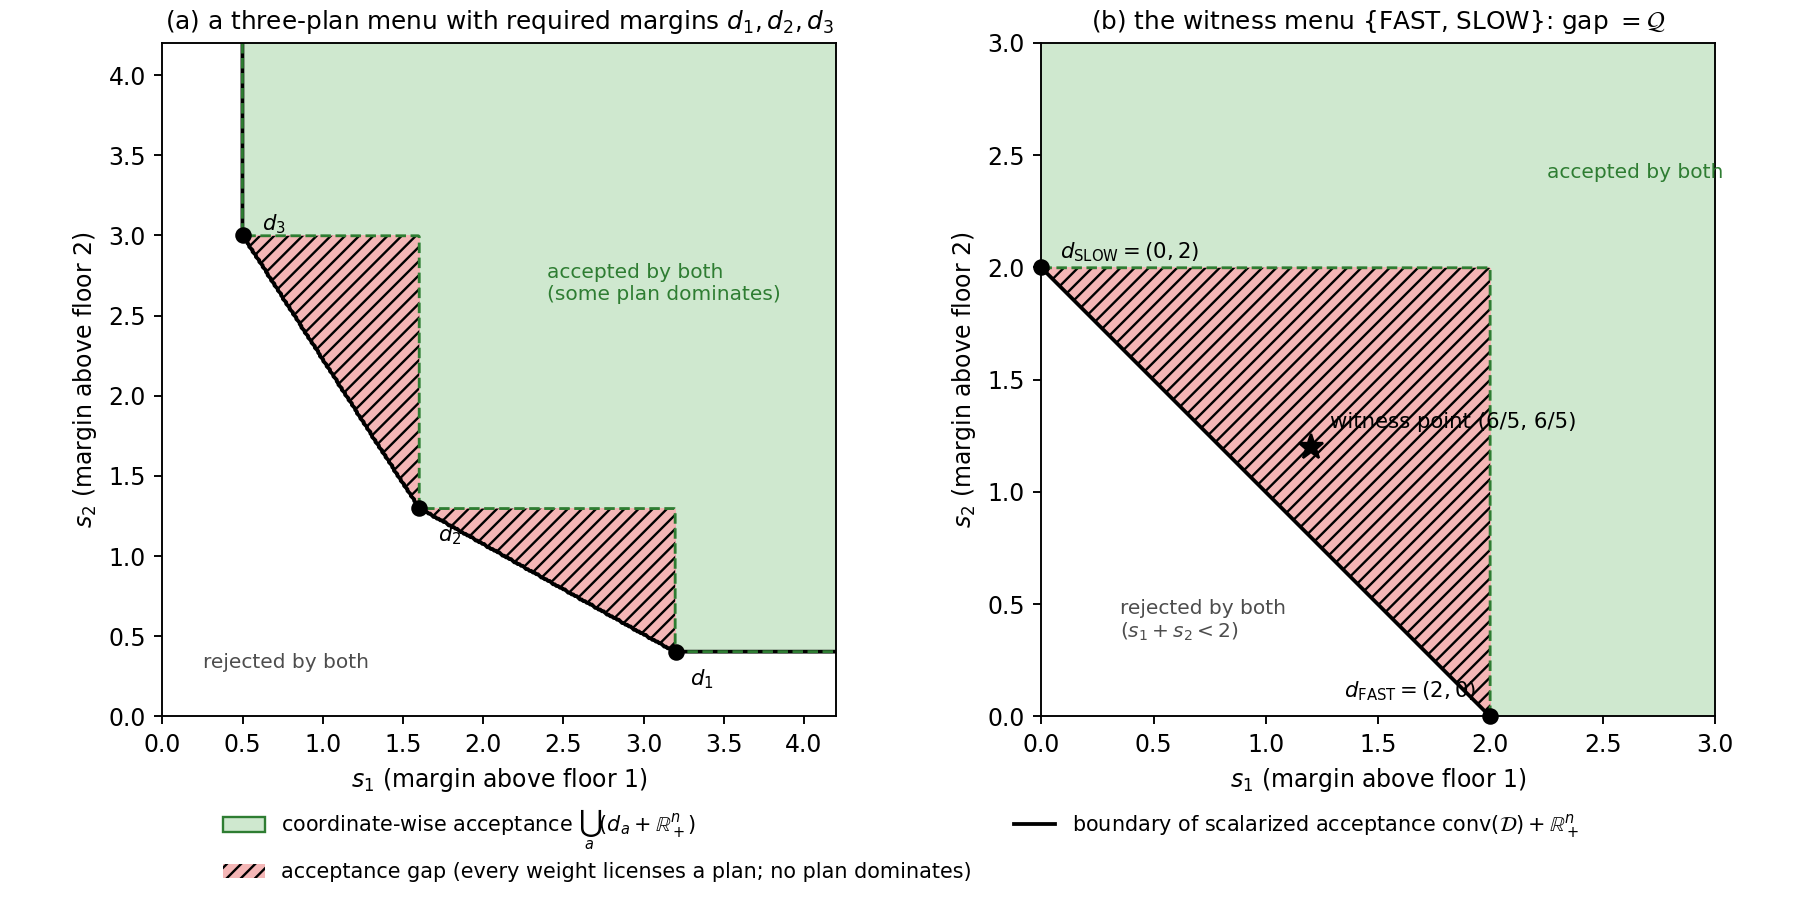
\includegraphics[width=\linewidth]{fig_finite_menu_geometry.png}
\caption{The finite-menu geometric characterisation (Theorem~\ref{thm:menu}) in the plane of two floor margins. Green: coordinate-wise acceptance, the union of the orthants $d_a+\mathbb R^2_+$ (some plan dominates). Black boundary: scalarized acceptance, $\conv(\mathcal D)+\mathbb R^2_+$. Hatched: the acceptance gap, where every weighting licenses some plan but no single plan keeps every floor. (a) A three-plan menu. (b) The margin-class plans of the witness datum, $d_{\textsc{fast}}=(2,0)$ and $d_{\textsc{slow}}=(0,2)$: the gap is the discrepancy triangle $\Q=\{s_1<2,\,s_2<2,\,s_1+s_2\ge2\}$ of Theorem~\ref{thm:witness}, with the witness point $(6/5,6/5)$ in its interior; the reserve-financed plan, which is outside the margin class, serves the triangle only when the reserve covers its cost.}
\label{fig:geometry}
\end{figure}

\section{An explicit witness: the separation on a rational datum}\label{sec:witness}

\subsection{The witness datum}\label{sec:datum}

Two architectures -- extraction ($q=0$) and regeneration ($q=1$) -- share one review interval $[0,1]$. The phase state is $(q,x,s_1,s_2)$: a physical reserve stock $x$ (a bridge stock, for instance an adjustment fund) and two typed floors $s_1$ and $s_2$ normalised at zero (on the benchmark of Section~\ref{sec:benchmark}: a biomass margin above a limit reference point and a fleet income margin). The transition-safe set is $S_0=\{x\ge0,\ s_1\ge0,\ s_2\ge0\}$ and the destination set is $G=\{(1,x,s):x\ge0,\ s\ge0\}$, with destination maintainability witnessed by a hold policy. The reset adds the strictly positive gain $e=(\tfrac14,\tfrac14)$, placing successors in the interior of $G$. The rescue cost is $c=1$. Initial states are $X_0=\{(0,x,s):x\ge0,\ s\ge0\}$.

Four plans are available (Table~\ref{tab:actions}), written as piecewise-linear maps on the breakpoints $\{0,\tfrac12,1\}$ and monotone on each piece, so that every tube is the exact visited set. The disturbance class is \emph{action-indexed}: the adverse disturbance triggers the worst-case dip, of fixed depth $2$, in the active plan's characteristic coordinate ($s_1$ for \act{fast}, $s_2$ for \act{slow}); on the benchmark the depth $2$ is a quota pulse of $3/2$ plus an environmental shock of $1/2$. The worst-case tube of \act{fast} is therefore $[s_1-2,s_1]$ in $s_1$ with $s_2$ and $x$ constant, that of \act{slow} is symmetric, and that of \act{staged} is $[x-1,x]$ in $x$ with both floors nondecreasing. A shared-shock class, in which the environmental component strikes every plan, is treated in Section~\ref{sec:commonshock}.

\begin{table}[!htbp]
\centering\small
\caption{The plan menu of the witness datum from an initial state $(0,x,s)$, $x\ge0$, $s\ge0$. Trajectories are worst-case; $e=(\tfrac14,\tfrac14)$.}
\label{tab:actions}
\begin{tabularx}{\textwidth}{@{}lXl@{}}
\toprule
Plan & Within-interval trajectory (worst case) & Successor \\
\midrule
\act{no-switch} & state constant & $\{(0,x,s)\}$ -- misses $G$ \\
\act{fast} & $s_1(t)=s_1-4t$ on $[0,\tfrac12]$, $s_1-4(1-t)$ on $[\tfrac12,1]$; $s_2,x$ constant & $\{(1,x,s+e)\}$ \\
\act{slow} & $s_2(t)=s_2-4t$ on $[0,\tfrac12]$, $s_2-4(1-t)$ on $[\tfrac12,1]$; $s_1,x$ constant & $\{(1,x,s+e)\}$ \\
\act{staged} & $x(t)=x-t$ on $[0,1]$; floors grow linearly to $s+e$ & $\{(1,x-1,s+e)\}$ \\
\bottomrule
\end{tabularx}
\end{table}

\noindent\textit{Role of \act{no-switch}.} \act{no-switch} is the status-quo, non-transition baseline: its successor keeps $q=0$ and therefore misses the destination set $G$. It remains in the four-action menu so that this failure is explicit; \act{fast}, \act{slow} and \act{staged} are the candidate transition plans.

The datum is deliberately spare. Its margin-class plans are \act{fast} and \act{slow}, with $\mathcal D=\{(2,0),(0,2)\}$, so Theorem~\ref{thm:menu} predicts the gap $\{s_1+s_2\ge2\}\setminus(\{s_1\ge2\}\cup\{s_2\ge2\})$ among them; \act{staged} lies outside the margin class, because its admissibility is governed by the reserve rather than by the floors, and it is what splits the predicted gap into a rescuable and an impossible part.

\subsection{The witnessed separation}

\begin{theorem}[witnessed separation]\label{thm:witness}
On the witness datum, over $X_0$:
\begin{enumerate}[label=\textup{(\arabic*)},leftmargin=2em]
\item $\Vtyp=\{x\ge1\}\cup\{s_1\ge2\}\cup\{s_2\ge2\}$.
\item $\Vweak=\bigcap_{w\in\Wp}\mathcal V_w=\{x\ge1\}\cup\{s_1+s_2\ge2\}$.
\item $\Vphys=\Vend=X_0$.
\end{enumerate}
Define the \emph{discrepancy region} $\Q=\{s_1<2,\ s_2<2,\ s_1+s_2\ge2\}$ ($x$ unrestricted), the \emph{rescue set} $R=\Q\cap\{x\ge1\}$ and the \emph{impossibility region} $I=\Q\cap\{x<1\}$. Then:
\begin{enumerate}[label=\textup{(\arabic*)},leftmargin=2em,resume]
\item $\FP=\Vweak\setminus\Vtyp=I$. The acceptance gap is exactly the impossibility region; it is nonempty, with relative interior $\{0<x<1,\ 0<s_1<2,\ 0<s_2<2,\ s_1+s_2>2\}$ in the $q=0$ slice. The rescue set $R$ lies in $\Vtyp$, not in the gap.
\item Both hierarchy inclusions are strict: every point of $I$ lies in $\Vweak\setminus\Vtyp$, and $(x,s_1,s_2)=(\tfrac12,\tfrac1{10},\tfrac1{10})$ lies in $\Vphys\setminus\Vweak$.
\item \textup{(Per-weight plan disagreement.)} On the relative interior of $\Q$ ($0<s_2<2$), for weights with $w_1>0$ put $r=w_2/w_1$. Then \act{fast} is licensed exactly for $r\ge\rho_1$ and \act{slow} exactly for $r\le\rho_2$, where
\[
\rho_1=\frac{2-s_1}{s_2},\qquad \rho_2=\frac{s_1}{2-s_2},\qquad \rho_2\ge\rho_1\iff s_1+s_2\ge2 .
\]
Among the two principal plans, $r>\rho_2$ licenses \act{fast} but not \act{slow}, $r<\rho_1$ licenses \act{slow} but not \act{fast}, and both are licensed for $\rho_1\le r\le\rho_2$. The axis weights are covered separately: $(1,0)$ licenses \act{slow} but not \act{fast}, while $(0,1)$ licenses \act{fast} but not \act{slow}, among those two plans. On $I$ no single plan serves every weight: $\bigcap_wE_w(z)=\Etyp(z)=\varnothing$. On $R$, \act{staged} is typed-admissible and serves every weight.
\item \textup{(The rescue split.)} $R$ is typed-transformable, witnessed by \act{staged}: bridging at cost $c=1$ keeps both floors intact and lands in $G$. $I$ is aggregate-feasible for every cone weight yet admits no typed-admissible plan, with four exhibited violations: \act{fast} breaches the $s_1$ floor under its adverse disturbance, \act{slow} the $s_2$ floor, \act{staged} drives $x$ negative, and \act{no-switch} misses $G$.
\end{enumerate}
\end{theorem}

The proof is in \ref{app:witness}; the formulas for $\rho_1,\rho_2$ require $0<s_2<2$, and the ratio is used for $w_1>0$; the two coordinate-axis weights are classified directly in part (6). On boundary faces in the state coordinates, the classification follows from the closed-set identities (1)--(2). Table~\ref{tab:regions} records the two verdicts region by region, and Figures~\ref{fig:triangle} and \ref{fig:paths} display them.

\paragraph{The witness point} At $(x,s_1,s_2)=(\tfrac12,\tfrac65,\tfrac65)$, the aggregate passes ($\tfrac{12}5\ge2$) but no menu plan is typed-admissible. The thresholds $(\rho_1,\rho_2)=(\tfrac23,\tfrac32)$ give \act{slow}-only, both, and \act{fast}-only licensing at $r=\tfrac12,1,2$, respectively. At $x=1$, \act{staged} rescues the same floors.

\paragraph{Reading} The compensatory assessment's binding condition is a total budget, $s_1+s_2\ge2$; the noncompensatory assessment requires either one floor to survive its own worst-case dip ($s_i\ge2$) or the reserve to cover the rescue cost ($x\ge1$). Between the two conditions the compensatory doctrine certifies -- per weight, with weight-dependent plans -- transitions the noncompensatory doctrine rejects, and the aggregate reading cannot tell $I$ from $R$: the two differ only in $x$, which the index does not see. Part (7) is a \emph{negative certificate} in the sense of a rejection with an exhibited violated constraint for each plan, exhausting the menu; it is a complete verdict relative to the menu, not an inconclusive one.

\begin{table}[!htbp]
\centering\small
\caption{Region dictionary on the witness datum (Theorem~\ref{thm:witness}).}
\label{tab:regions}
\begin{tabularx}{\textwidth}{@{}>{\raggedright\arraybackslash}p{0.30\textwidth}>{\raggedright\arraybackslash}p{0.17\textwidth}>{\raggedright\arraybackslash}p{0.14\textwidth}X@{}}
\toprule
Region & Per-weight verdict & Common-plan verdict & Reason \\
\midrule
$x\ge1$, all $s$ & accept & accept & \act{staged} serves every weight \\
$s_1\ge2$ or $s_2\ge2$ & accept & accept & \act{fast}/\act{slow} survives its own dip \\
$R$: $x\ge1$, $s_1<2$, $s_2<2$, $s_1+s_2\ge2$ & accept & accept & the reserve finances \act{staged} \\
$I$: $x<1$, $s_1<2$, $s_2<2$, $s_1+s_2\ge2$ & accept (weight-dependent plans) & reject & dips breach the floors; the reserve cannot finance phasing \\
$x<1$, $s_1+s_2<2$ & reject & reject & even the aggregate rejects \\
\bottomrule
\end{tabularx}
\end{table}

\begin{figure}[!htbp]
\centering
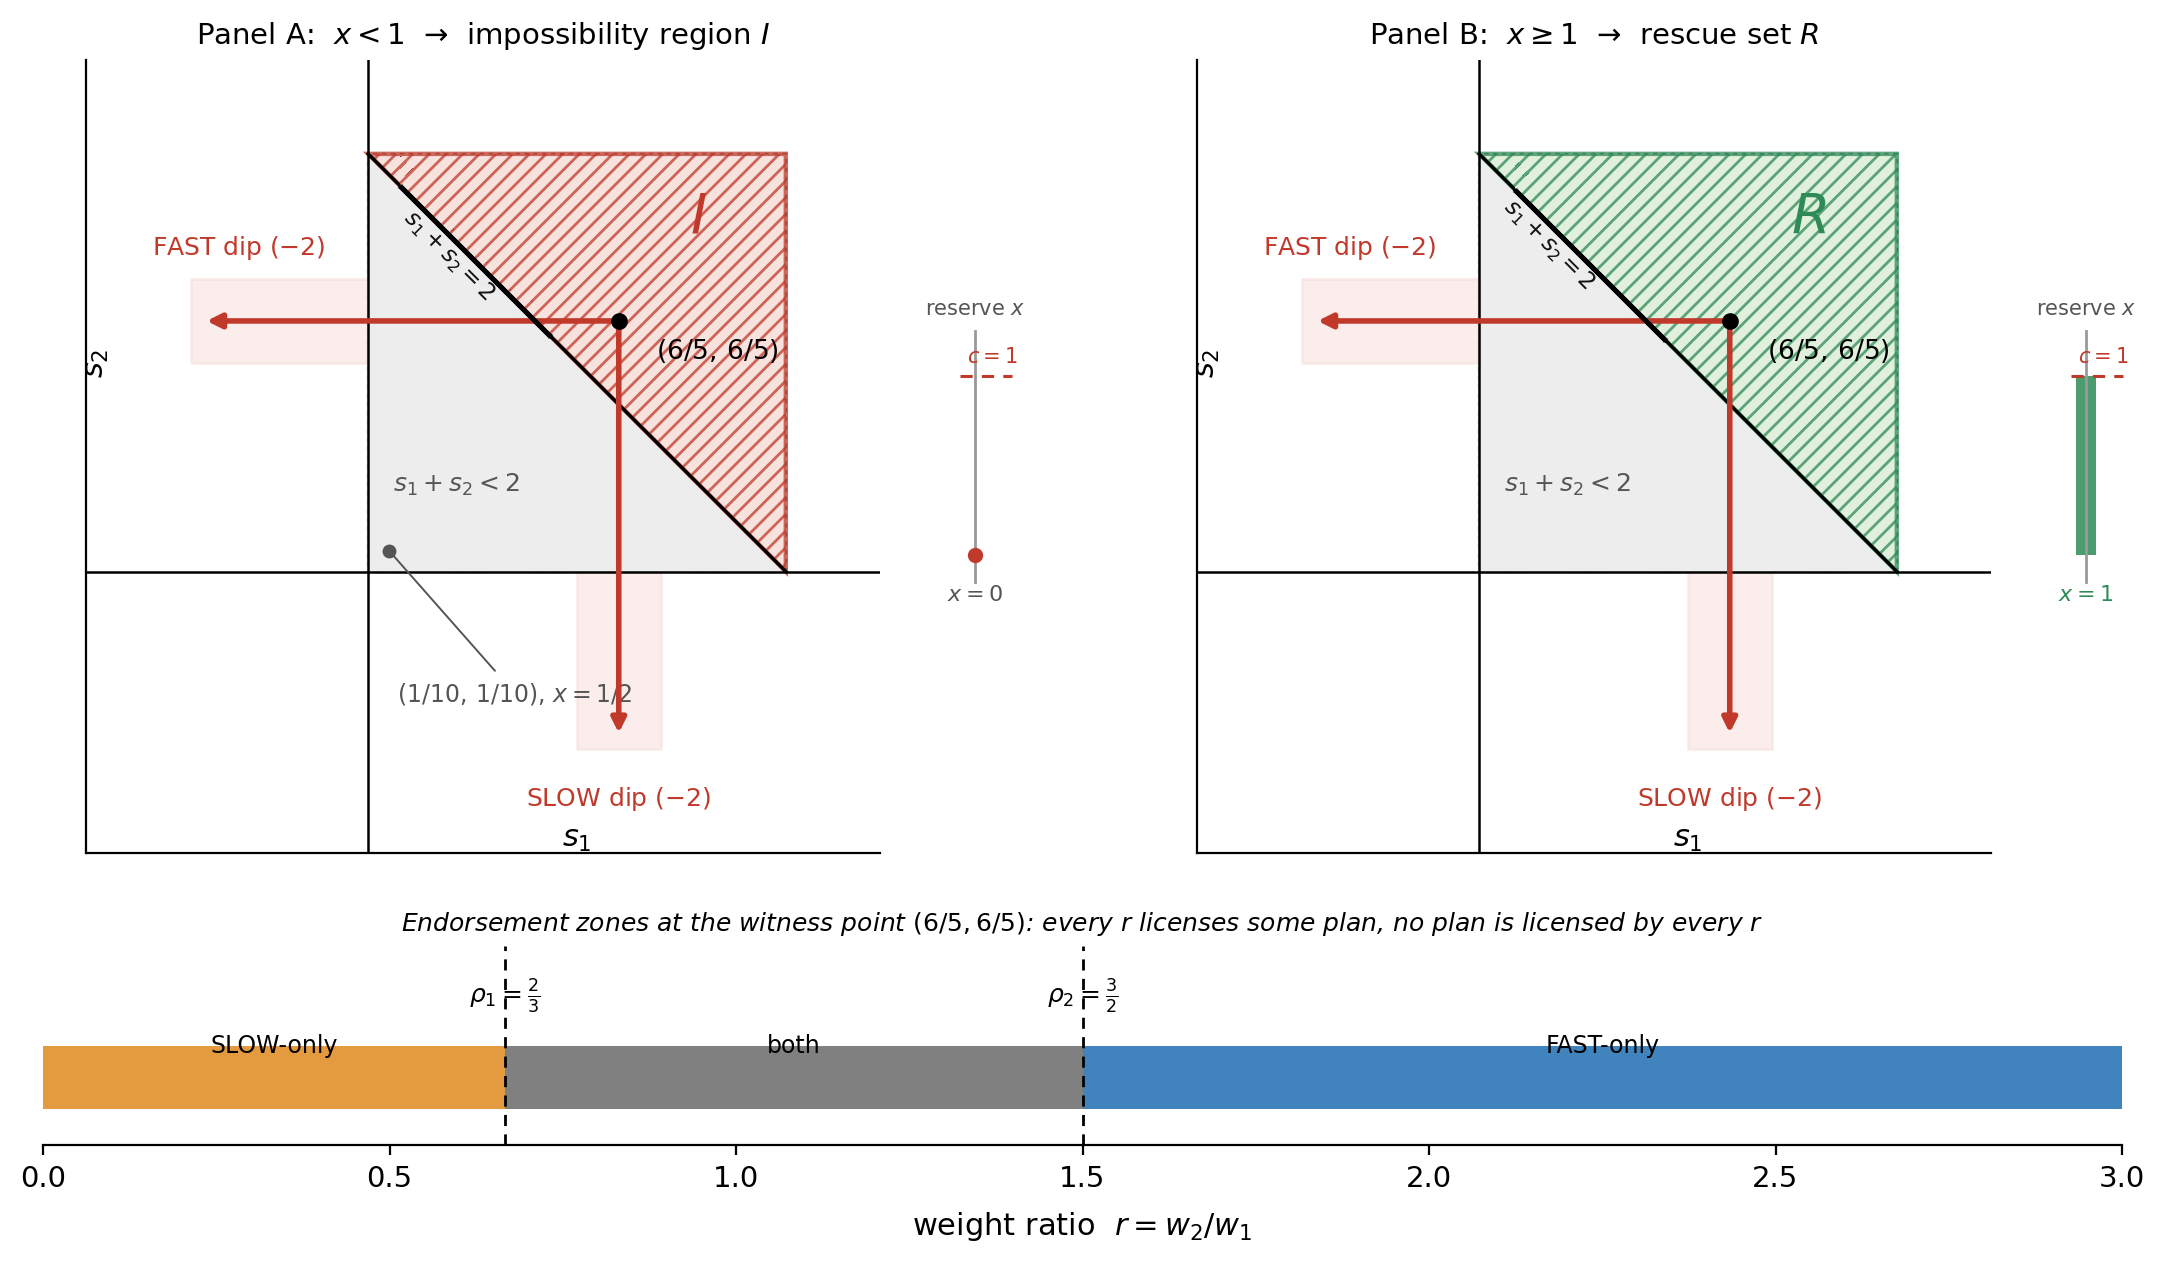
\includegraphics[width=\linewidth]{fig_witness_triangle.png}
\caption{The discrepancy triangle $\Q=\{s_1<2,\ s_2<2,\ s_1+s_2\ge2\}$ in the floor plane. Panel A ($x<1$): $\Q$ is the impossibility region $I=\FP$; the arrows show the worst-case dips of \act{fast} ($s_1\to s_1-2$) and \act{slow} ($s_2\to s_2-2$) crossing the floors from the witness point $(6/5,6/5)$, and the point $(1/10,1/10)$ is the second strictness witness. Panel B ($x\ge1$): the same triangle is the rescue set $R$, served by \act{staged}. Below the diagonal both assessments reject when $x<1$ and accept when $x\ge1$. The reserve bars show the bridge stock against the rescue cost $c=1$ at representative slices ($x=0$ and $x=1$; the witness point sits at $x=\tfrac12$). The bottom strip gives the licensing zones at the witness point: \act{slow} only for $r<\rho_1=\tfrac23$, both for $\tfrac23\le r\le\tfrac32$, \act{fast} only for $r>\rho_2=\tfrac32$.}
\label{fig:triangle}
\end{figure}

\begin{figure}[!htbp]
\centering
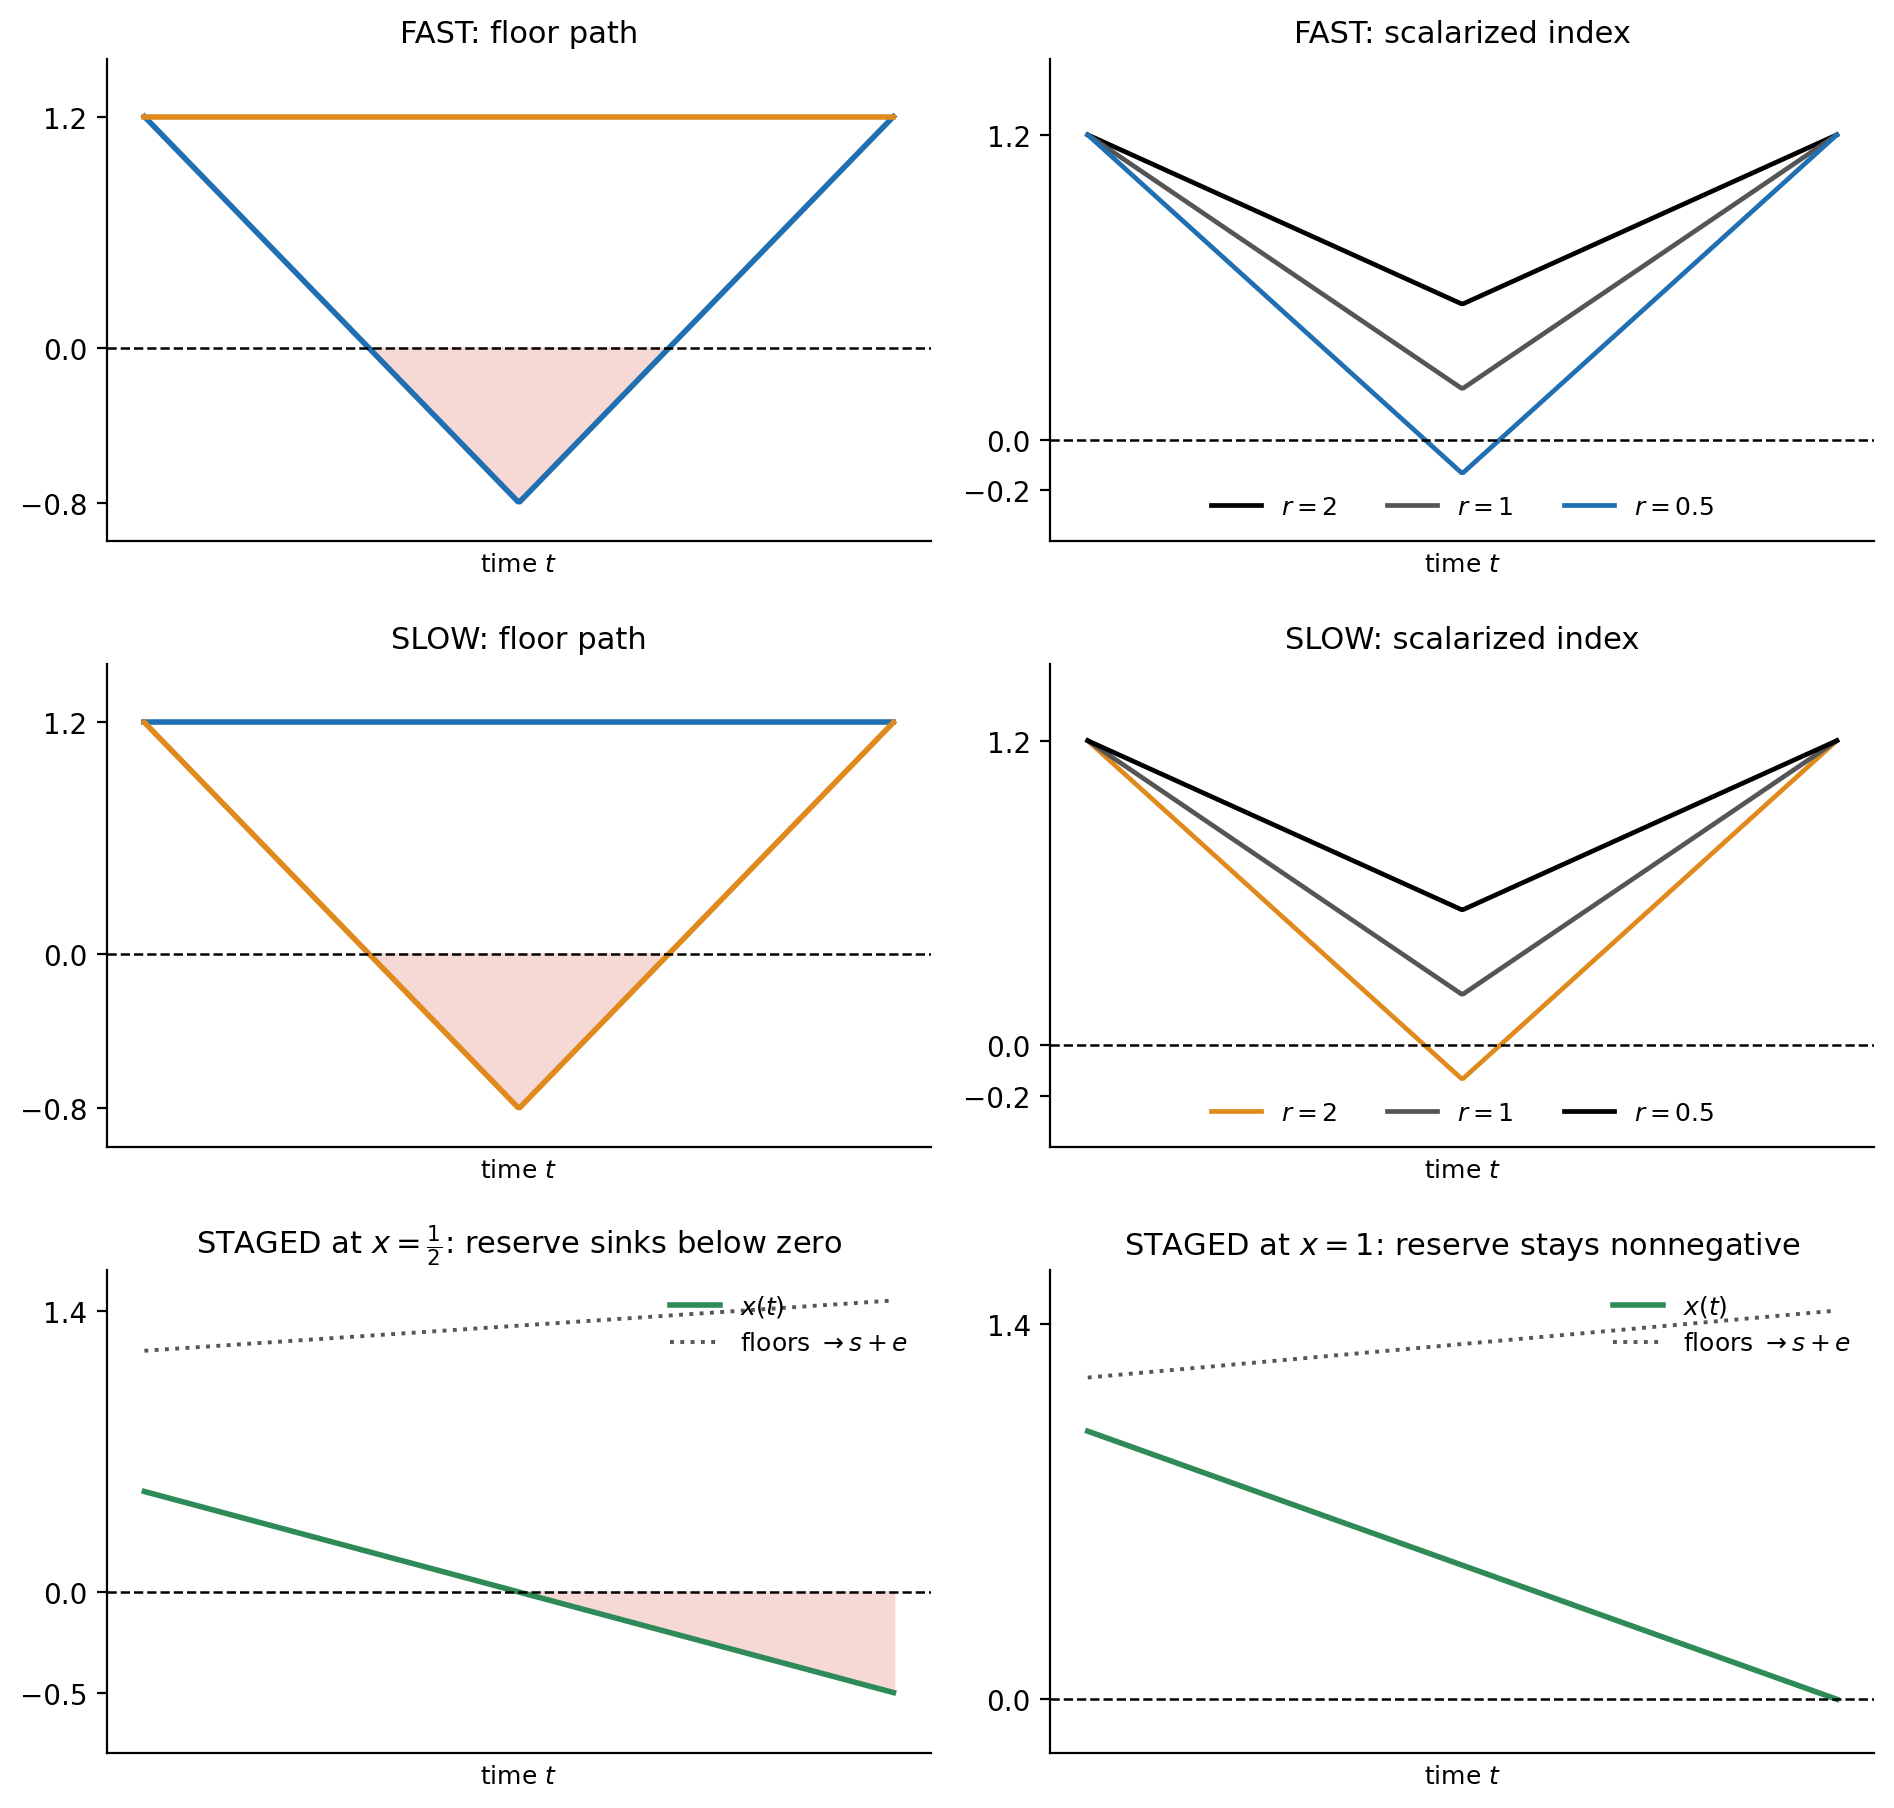
\includegraphics[width=0.9\linewidth]{fig_path_view.png}
\caption{Path view at the witness point under the worst-case disturbance. Rows: \act{fast}, \act{slow}, \act{staged}. Left: the floor paths (solid) against the zero floor (dashed). Right: the scalarized index $s_1+rs_2$ for $r\in\{2,1,\tfrac12\}$. Under \act{fast} the index stays nonnegative for $r=2$ and $r=1$ while $s_1$ breaches its floor; under \act{slow} the mirror holds. The only plan that protects both floors, \act{staged}, consumes the reserve linearly: infeasible at $x=\tfrac12$, feasible at $x=1$ -- the difference between $I$ and $R$.}
\label{fig:paths}
\end{figure}

\clearpage
\subsection{Persistence under horizon extension, and its limit}\label{sec:persist}

Is the one-interval separation an artefact of the one-interval framing? Two results delimit the answer.

\begin{proposition}[persistence and erasure]\label{prop:persist}
\textup{(i)} Extend the witness datum to $m\ge2$ review intervals by prepending hold intervals, with sole prefix action \act{hold} (tube $\{z\}$, successor $\{z\}$, safe set $S_0$) available at every prefix state, unchanged terminal and successor architecture, and no additional reset or disturbance branches. Then for every stage $j$, $\mathcal V^{\mathrm{typ}}_j\subseteq\bigcap_{w}\mathcal V^{w}_j\subseteq\mathcal V^{\mathrm{phys}}_j$, the stage-0 accepted regions are the witness regions pulled back through the holds, and both strictness witnesses of Theorem~\ref{thm:witness}(5) persist.
\textup{(ii)} Persistence is architecture-conditional: there is a two-interval datum whose single-interval truncation exhibits an acceptance gap and whose two-stage extension erases it. The same final typed and scalarized terminal rules are used in both versions; in the extension, a repair stage enlarges the stage-1 successor accepted sets to the whole state space, while the stage-1 tubes themselves remain safe.
\end{proposition}

The erasure datum of (ii) (SI~S2.2) has two floors, no reserve, and a first stage with two actions that transfer one unit from one floor to the other. At $(2/5,2/5)$, the one-stage version is weak-accepted for every weight (the actions are licensed for $r\ge3/7$ and $r\le7/3$) but typed-rejected. In the two-stage version the first-stage tubes stay in the nonnegative orthant, and a second-stage repair sends every successor to $(1,1)$, so both stage-1 accepted sets are all of $\mathbb R^2$; the original final typed and scalarized terminal rules are unchanged. The witness datum itself is not erased this way: on $I$ its plans violate the stage-local path constraint, which a later action cannot undo. The example shows one sufficient repair-stage mechanism, not a general erasure rule: safe continuation cannot repair an earlier tube breach, and equality of terminal sets or action coupling alone does not imply alignment of the pathwise constraints.

\subsection{What closes the gap and what does not}\label{sec:closing}

Under the witness's declared linear-flow extension, the physical convexification instrument is the \emph{closed blend family}: for $\delta\in[0,1]$, $\act{blend}_\delta$ uses the fractional control $u_\delta=\delta\,u_{\act{fast}}+(1-\delta)\,u_{\act{slow}}$. Its endpoints are the primitive plans, and its worst-case tube and successor are the corresponding convex combinations under the stated linearity assumption. This physical blend is stronger than abstract convexification of required-margin vectors; an application must demonstrate it from model equations or declare it as a management assumption (for example, fractional effort or quota allocation with monitoring and enforcement).

\begin{theorem}[blend collapse]\label{thm:blend}
On the witness datum, over $X_0$:
\begin{enumerate}[label=\textup{(\roman*)},leftmargin=2em]
\item $\act{blend}_\delta$ is typed-admissible at $z$ exactly when $\delta\in\big[\,1-\tfrac{s_2}2,\ \tfrac{s_1}2\,\big]\cap[0,1]$, an interval nonempty exactly when $s_1+s_2\ge2$ (a singleton at equality), independent of $x\ge0$ and of the weight;
\item the typed accepted set of the menu augmented by the blend family is exactly the compensatory region,
$\Vtyp^{\mathrm{blend}}=\{x\ge1\}\cup\{s_1+s_2\ge2\}=\Vweak$: the gap vanishes, and the blend family reaches nothing beyond $\Vweak$;
\item the admissible window depends on the state through $(s_1,s_2)$ alone, so a single $\delta$ serves every weight: on $I$ the blend is the common plan that no member of the finite menu supplies.
\end{enumerate}
\end{theorem}

\begin{proposition}[complete-excursion concatenation preserves primitive floor violations]\label{prop:timeshare}
Consider the control extension in which a sequential policy is required to execute each selected primitive at full strength for its complete unit-interval excursion, with visited set exactly the union of the corresponding primitive worst-case tubes. Within this specified class, a policy that uses both \act{fast} and \act{slow} is typed-admissible if and only if $s_1\ge2$ and $s_2\ge2$. Thus no such complete-excursion concatenation is typed-admissible on $I$.
\end{proposition}

This proposition is conditional on the stipulated union-of-complete-tubes semantics; it is not a theorem about ordinary finite-rate switching. For example, in the no-shock branch of a natural full-rate derivative extension $\dot s_1=-4$ before $t=1/2$ and $+4$ after for \act{fast}, with the analogous rates on $s_2$ for \act{slow}, the schedule fast on $[0,1/4]$, slow on $[1/4,1/2]$, fast on $[1/2,3/4]$, and slow on $[3/4,1]$ takes $(6/5,6/5)$ through $(1/5,6/5)$, $(1/5,1/5)$, $(6/5,1/5)$, and back to $(6/5,6/5)$. Both floors remain positive with three switches. This is a different admissible-control extension, not a counterexample to the conditional proposition.

The two results compare distinct declared control extensions. Under action-indexed disturbances and linear fractional flows, the blend family closes the typed gap exactly on $s_1+s_2\ge2$. Under the shared-shock class of Section~\ref{sec:commonshock}, the blend window instead requires $s_1+s_2\ge5/2$, so it is empty at the canonical point $s_1+s_2=12/5$ (Proposition~\ref{prop:commonshock}). The complete-excursion result concerns only a policy whose visited set is the union of both full primitive tubes; the three-switch example above demonstrates a different implementation. Neither statement identifies physical blending with a lottery over plans or ranks all admissible switching policies.

The remaining instrument acts on the reserve. Define the augmentation map $\mathsf{Aug}_\kappa:(x,s,\mathcal A)\mapsto(x+\kappa,\ s,\ \mathcal A\cup\{\act{staged}_\kappa\})$, where $\act{staged}_\kappa$ is \act{staged} run from the augmented reserve, and the \emph{rescue threshold} $\kappa^*(z)=\inf\{\kappa\ge0:\ \exists a\in\mathcal A_\kappa,\ a\in\Etyp(z)\}$. The augmented state is $(x+\kappa,s_1,s_2)$, so increasing $\kappa$ changes only the available reserve.

\begin{proposition}[rescue threshold]\label{prop:rescue}
On the witness datum, for every $z\in X_0$,
\[
\kappa^*(z)=(1-x)_+\cdot\mathbf 1[\,x<1,\ s_1<2,\ s_2<2\,]=(1-x)\cdot\mathbf 1[\,z\notin\Vtyp\,].
\]
\end{proposition}

On $I$ the threshold is $1-x>0$; on $R$ and on all of $\Vtyp$ it is $0$. Because $\act{staged}_\kappa$ is admissible exactly when $x+\kappa\ge1$, independently of the floors, the reserve route admits every state of the failure set $\{x<1,s_1<2,s_2<2\}$ at cost $1-x$ -- including states such as $(\tfrac12,\tfrac1{10},\tfrac1{10})$ that even the aggregate rejects; $I$ is the part of the failure set on which the aggregate still certifies. Along this route the distance to the feasible slice $\{x\ge1\}$ equals the violation $(1-x)_+$ itself, so the error-bound modulus \citep{Fabian2010} of the relation is identically $1$: the route is perfectly conditioned. Table~\ref{tab:instruments} summarises how the instruments act on the gap.

\begin{table}[!htbp]
\centering\small
\caption{Instruments acting on the acceptance gap.}
\label{tab:instruments}
\begin{tabularx}{\textwidth}{@{}>{\raggedright\arraybackslash}p{0.24\textwidth}>{\raggedright\arraybackslash}p{0.32\textwidth}X@{}}
\toprule
Instrument & Operation & Effect on the gap \\
\midrule
Reweighting & change $w$ & none: the gap is a statement over all $w$ \\
Restricting the weight family & replace $\Wp$ by $W\subset\Wp$ & $\mathcal V_W$ can only expand while $\Vtyp$ is unchanged, so $\mathcal V_W\setminus\Vtyp$ can only expand (Proposition~\ref{prop:monotone}) \\
Reserve augmentation & add $\act{staged}_\kappa$, $x+\kappa\ge1$ & closes it where only the reserve binds, at cost $\kappa^*=1-x$ (Proposition~\ref{prop:rescue}) \\
Menu convexification & replace $\mathcal D$ by $\conv(\mathcal D)$ (blend family) & closes it exactly on the scalarized region (Theorems~\ref{thm:menu}, \ref{thm:blend}) \\
Discrete time-sharing & union of the primitive tubes & closes it only where both dips are separately survivable (Proposition~\ref{prop:timeshare}) \\
\bottomrule
\end{tabularx}
\end{table}

\subsection{Beyond linear aggregation: the substitutability ladder}\label{sec:ladder}

The results so far concern the linear index. We evaluate Protocol~2 on the witness under a normalized-margin CES family. Set $\lambda_i=1+s_i$ and, for normalized weights $w_i\ge0$, $\sum_iw_i=1$, define
\[
\begin{gathered}
M_\theta(\lambda;w)=\Big(\sum_iw_i\lambda_i^\theta\Big)^{1/\theta},\qquad \sigma=\frac1{1-\theta},\\
-\infty<\theta<1\quad(0\le\sigma<\infty),\qquad \theta=1\text{ corresponds to }\sigma=\infty.
\end{gathered}
\]
with the usual limits: $\theta=1$ is the linear aggregate, $\theta=0$ the geometric mean, $\theta=-1$ the harmonic mean, and $\theta\to-\infty$ the weighted support minimum. The inputs $\lambda_i$ are constructed normalized-margin indices; they are not automatically physical abundance ratios. A state is accepted at rung $\theta$ when every weight has some menu plan satisfying $M_\theta\ge1$ along its worst-case tube, subject to the same physical and destination constraints. We impose an additional floor-safety convention: for every $\theta<1$, a plan is rejected if any tube coordinate has $\lambda_i\le0$, regardless of the weight. This is not an inherent property of every CES mean: for $0<\theta<1$, a zero input can still yield a positive mean, while negative inputs are outside the standard geometric-mean domain. The convention makes any collapsed floor coordinate independently disqualifying; the linear member alone is allowed to compensate across it. At $\theta=1$, $M_1\ge1$ is exactly $w\cdot s\ge0$, so the original compensatory protocol and its licensing thresholds are recovered. At the Leontief limit, $M_{-\infty}$ is the minimum over the positive-weight support. A strictly positive full-support weight therefore requires every coordinate to meet its floor along the tube, while typed safety passes every support minimum; hence the all-weight acceptance set is exactly the typed set.

On the gap-region diagonal $z=(x<1,s,s)$, $s\in(1,2)$, the per-weight cover condition reduces, by the symmetry of the two principal plans, to a single comparison at the equal weight: accept iff $(s-1)^\theta+(s+1)^\theta\ge2$ for $\theta>0$, iff $s^2\ge2$ for $\theta=0$, and iff $(s-1)^\theta+(s+1)^\theta\le2$ for $\theta<0$. Each rung therefore has an exact critical floor $s^*(\theta)$, and the critical floors form a ladder (Table~\ref{tab:ladder}, Figure~\ref{fig:ladder}).

\begin{theorem}[the substitutability ladder]\label{thm:ladder}
On the witness datum:
\begin{enumerate}[label=\textup{(\roman*)},leftmargin=2em]
\item \textup{(Nesting.)} For rungs $\theta>\theta'$ and every state, acceptance at $\theta'$ implies acceptance at $\theta$. The accepted rungs at each state form a prefix of the ladder, so the \emph{critical elasticity} $\sigma^*(z)=\inf\{\sigma:\ z\text{ accepted at }\sigma\}$ is well defined; it is strictly positive and finite on every gap state in the deep interior ($1<s_1<2$ and $1<s_2<2$), where the finite primitive menu has positive tube ratios and the scalarized margin is strict at every normalised weight; it is equal to $\infty$ on gap states with $\min(s_1,s_2)\le1$, for which only the linear member certifies. Boundary equalities are not covered by the strictness assertion.
\item \textup{(Pointwise.)} For every gap state in the strict interior of the floor-margin region ($0<s_1<2$, $0<s_2<2$, $s_1+s_2>2$), some strictly positive elasticity rejects it, so the Leontief limit is not needed to reject a fixed interior gap state. On the deep-interior subset ($1<s_1<2$ and $1<s_2<2$), a finite rung below the linear member still accepts the state. Gap states with $\min(s_1,s_2)\le1$ are accepted at the linear member only.
\item \textup{(Uniform on the diagonal slice.)} For every $\theta<1$ the rung falsely certifies an exact interval $[s^*(\theta),2)$ of the witness-defined diagonal gap states, with $s^*(\theta)<2$ strictly; for the displayed rungs the critical floors increase as elasticity falls: $1<\sqrt{6\sqrt3-9}<5/4<\sqrt2<\varphi<\sqrt3<\cdots\to2$ (Table~\ref{tab:ladder}), approaching the typed boundary. Thus no positive elasticity is uniformly safe even over the full gap (the diagonal intervals alone witness failure), $\inf_{z\in\Q}\sigma^*(z)=0$, and the only uniformly safe member is $\sigma=0$ -- the Leontief member, which is exactly the typed operator ($\mathcal V^{0}=\Vtyp$).
\end{enumerate}
\end{theorem}

\begin{table}[!htbp]
\centering\small
\caption{The exact ladder on diagonal gap states $z=(x<1,s,s)$: acceptance condition and critical floor $s^*(\theta)$ per rung.}
\label{tab:ladder}
\begin{tabularx}{\textwidth}{@{}ll>{\raggedright\arraybackslash}p{0.4\textwidth}X@{}}
\toprule
$\theta$ & $\sigma$ & accept iff & critical floor $s^*(\theta)$ \\
\midrule
$1$ & $\infty$ & $s\ge1$ & $1$ \\
$2/3$ & $3$ & $s^2\ge3$, else $27(s^2-1)^2\ge(3-s^2)^3$ & root in $(117/100,\,59/50]$ \\
$1/2$ & $2$ & $s\ge5/4$ & $5/4$ \\
$0$ & $1$ & $s^2\ge2$ & $\sqrt2$ \\
$-1$ & $1/2$ & $s^2\ge s+1$ & $\varphi=(1+\sqrt5)/2$ ($8/5$ rejects, $13/8$ accepts) \\
$-2$ & $1/3$ & $s^2\ge3$ & $\sqrt3$ \\
$-m$ & $1/(m+1)$ & $(s-1)^m+(s+1)^m\le2(s^2-1)^m$ & increasing in $m$ \\
$-\infty$ & $0$ & $s\ge2$ & $2$: the typed boundary \\
\bottomrule
\end{tabularx}
\end{table}

\begin{figure}[!htbp]
\centering
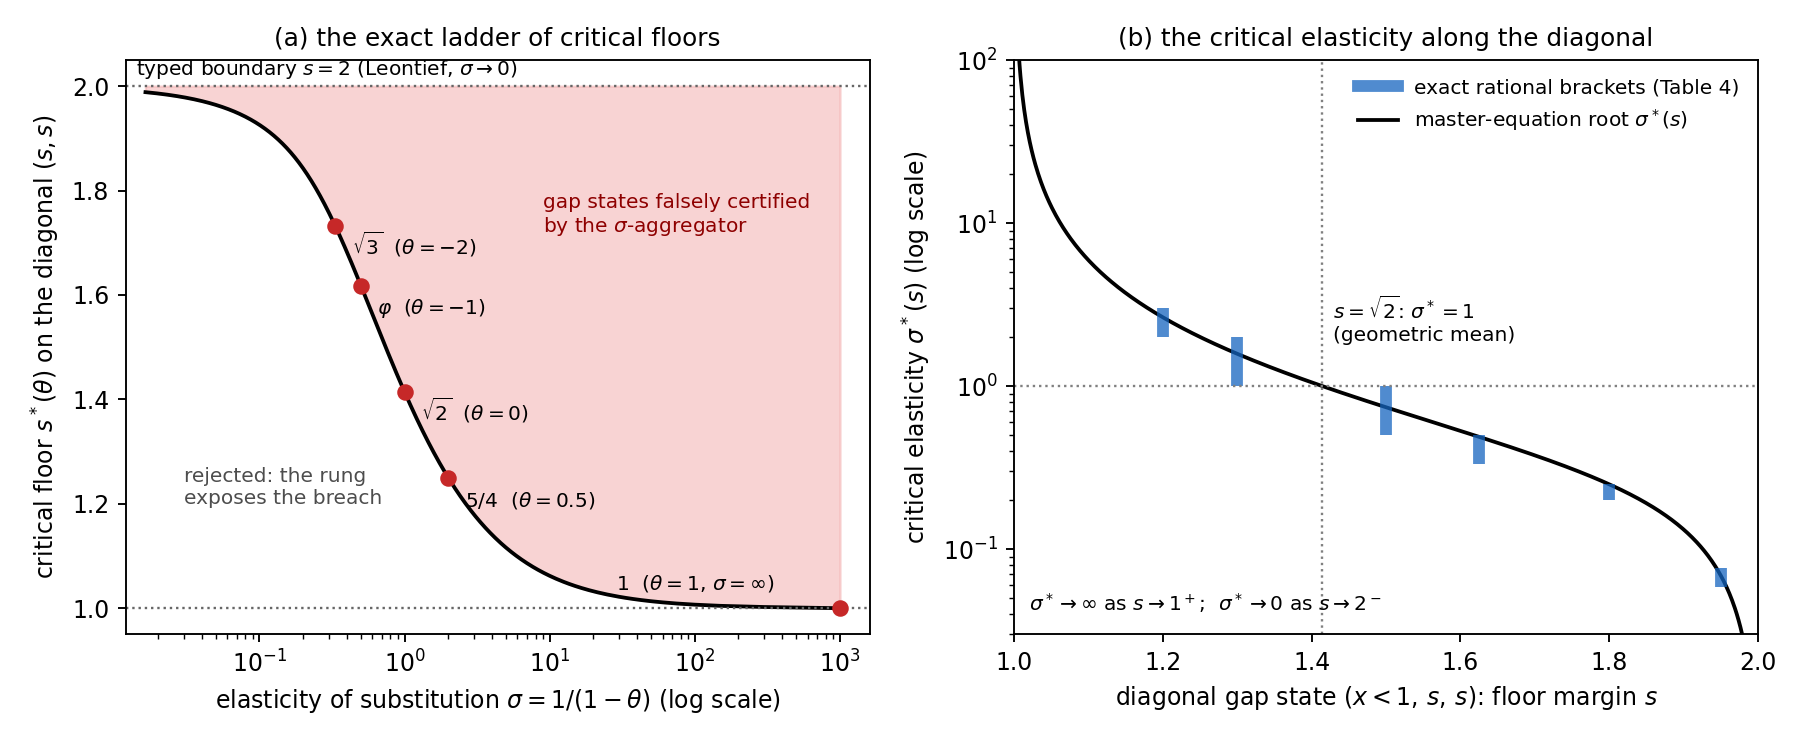
\includegraphics[width=\linewidth]{fig_substitutability_ladder.png}
\caption{The substitutability ladder (Theorem~\ref{thm:ladder}). (a) The critical floor $s^*(\theta)$ on the diagonal as a function of the elasticity $\sigma$; the shaded region above the curve is the set of diagonal gap states that the $\sigma$-aggregator falsely certifies. The exact algebraic rungs $1,\,5/4,\,\sqrt2,\,\varphi,\,\sqrt3$ are marked; the curve approaches the typed boundary $s=2$ only as $\sigma\to0$. (b) The critical elasticity $\sigma^*(s)$ along the diagonal (root of the master comparison), with the exact rational brackets of the deposited verifier overlaid: at the witness point $s=6/5$, $\sigma^*\in(2,3)$; at $s=5/4$, $\sigma^*=2$ exactly; $\sigma^*\to\infty$ as $s\to1^+$ and $\sigma^*\to0$ as $s\to2^-$.}
\label{fig:ladder}
\end{figure}

The theorem settles the objection in two scopes. Pointwise, the separation is not a Leontief phenomenon: at the witness point every aggregator with $\sigma\le2$ already rejects, and the floor-referenced dashboard value $(\lambda_1+\lambda_2)/2=(1/5+11/5)/2=6/5\ge1$ at the trough is contradicted by the geometric index $\sqrt{11/25}<1$. Here $\lambda_i=1+s_i$, so $(\lambda_1+\lambda_2)/2=1+(s_1+s_2)/2$ is tested against $1$. Section~\ref{sec:benchmark} reports the same verdict in floor-margin coordinates as the unnormalised sum $s_1+s_2$ at threshold $0$: for normalized equal weights $w=(1/2,1/2)$, this sum is twice $w\cdot s$, so the rescaling does not change acceptance. Uniformly on the witness-defined diagonal gap slice, for every positive elasticity there are gap states arbitrarily close to the typed boundary that the aggregator certifies and no plan completes safely. The appearance of $\sqrt2$, $\varphi$ and $\sqrt3$ as the exact critical floors of the geometric, harmonic and $\sigma=1/3$ members is, to our knowledge, a new exact witness for the substitutability debate. Off the diagonal, the geometric-member comparison has the exact criterion in SI~S3.2, with boundary $s_2=\rho(s_1)$. The finite-grid and numerical fixed-sum explorations in SI~S3 do not establish a global slice-minimum or stationary-point theorem, and no such global claim is used here. The identification of the $\theta=0$ member with the Living Planet Index is at the level of functional form only: published LPI inputs and weighting are not Protocol~2, and the constructed inputs $\lambda_i=1+s_i$ depend on the chosen positive normalization of each margin. Under the optional biomass scale map in Section~\ref{sec:benchmark}, $B_m/B_{\mathrm{lim}}=1+s_1/2$, not $1+s_1$; the index is therefore not a physical abundance ratio. The all-weights protocol is also more restrictive than acceptance at one specified published weight, so its false-acceptance exposure can be smaller.

\subsection{Beyond action-indexed disturbances: the common shock}\label{sec:commonshock}

A second objection is that the gap depends on the action-indexed disturbance convention, under which the adverse event strikes only the coordinate the active plan moves. Decompose the datum as on the benchmark: each principal plan's announced schedule is a mid-interval tent of depth $3/2$ in its characteristic coordinate, and each environmental event is a transient tent dip of depth $\delta$ in one floor coordinate (the datum's depth $2=3/2+1/2$ fixes $\delta=1/2$); \act{staged}'s floors grow linearly, so an event of depth $\delta$ dips a growing floor by $\max(0,\delta-1/8)$. Under the \emph{common-shock class} the two coordinate events are separate disturbances each of which strikes every plan -- a marine heatwave striking the same biomass coordinate regardless of which harvest plan is running.

\begin{proposition}[the common-shock verdict]\label{prop:commonshock}
Under the common-shock class at $\delta=1/2$:
\begin{enumerate}[label=\textup{(\roman*)},leftmargin=2em]
\item $\Vtyp^{\mathrm{cs}}=\{s_1\ge2,\ s_2\ge\tfrac12\}\cup\{s_2\ge2,\ s_1\ge\tfrac12\}\cup\{x\ge1,\ s_1\ge\tfrac38,\ s_2\ge\tfrac38\}$ and
$\Vweak^{\mathrm{cs}}=\{x<1,\ s_1\ge\tfrac12,\ s_2\ge\tfrac12,\ s_1+s_2\ge2\}\cup\{x\ge1,\ s_1\ge\tfrac38,\ s_2\ge\tfrac38\}$, so the gap
$\mathrm{FP}_{\mathrm{cs}}=\{x<1,\ \tfrac12\le s_1<2,\ \tfrac12\le s_2<2,\ s_1+s_2\ge2\}$
survives: it is the action-indexed gap $I$ reduced by the exact $1/2$-cut, nonempty with interior, and the witness point is a member. On the surviving region the licensing thresholds are unshifted.
\item The rescue threshold becomes a trichotomy: $\kappa^*_{\mathrm{cs}}=0$ on $\Vtyp^{\mathrm{cs}}$; $(1-x)_+$ on failure states with $\min(s_1,s_2)\ge\tfrac38$; and $+\infty$ on failure states with $\min(s_1,s_2)<\tfrac38$, which no reserve increment rescues (witness $(\tfrac12,\tfrac14,3)$).
\item The blend window is nonempty exactly on $\{s_1\ge\tfrac12,\ s_2\ge\tfrac12,\ s_1+s_2\ge\tfrac52\}$, so the common-shock gap is not blend-closed on the band $s_1+s_2\in[2,\tfrac52)$ (witness $(\tfrac12,1,1)$).
\end{enumerate}
\end{proposition}

The separation is not an artefact of the action-indexed convention: under the common-shock model the gap persists, reduced by the exact $1/2$-cut. The model's rescue set also changes: on failure states with $\min(s)<3/8$, no finite reserve increment certifies, while the staged route has the stated coordinate-floor requirement. These are conditional feasibility results for the specified menu and disturbance class, not operational prescriptions. The coupled class (one disturbance carrying both events), its depth dependence with exact boundary $\delta=5/4$, the relocation of the gap to larger floors at full magnitude, and the collapse of the separation under a replace reading in which every plan faces the same plan- and weight-independent dip are stated and proved in SI~S4; the mechanism of that replace-reading collapse is that a common plan- and weight-independent dip removes the weak test's advantage of weight-wise plan choice, so the per-weight cover reduces to the typed condition.

\subsection{Verification}\label{sec:verification}

The retained analytic results are proved in Appendix~\ref{app:general}, Appendix~\ref{app:witness}, and SI~S2--S4. Exact-integer and rational verifiers provide finite supporting checks only; their state grids and check lists do not establish continuum claims, and the availability of each script and log is stated in SI~S7 and Data Availability. The cited Lean module contains formalized algebraic witness components and selected CES rungs, but its own scope excludes the general real-exponent nesting, continuity/IVT transfer, and relative-interior argument used by the full continuum theorem. We therefore treat those steps as paper proofs, not as machine-checked Lean results. No Lean build was run for this v77 revision; SI~S7 records the claim-to-coverage limits and the version mismatch of the available deposits.

\section{A resource-transition reading of the datum}\label{sec:benchmark}

The witness is abstract by design. This section gives it a Schaefer-style biomass reading using synthetic \emph{model biomass units} (MBU), not a calibrated fishery model. Biomass dynamics are specified, but the income-margin and reserve coordinates are normalized illustrative states whose paths are stipulated by the witness; they are not calculated from prices, costs, or fleet accounts. Northern-cod data enter only through a separately declared historical scale comparison (full detail in SI~S5). No model parameter is estimated from those data, and no fit, forecast, validation, or empirical performance claim is made.

\paragraph{State variables and scales} Let $B_m(t)$ be biomass in MBU over one annual review interval $t\in[0,1]$, with Schaefer surplus production $\varsigma(B_m)=rB_m(1-B_m/K)$, $r=4\,\mathrm{yr}^{-1}$, $K=10$ MBU, and model floor $B_{\mathrm{lim}}=2$ MBU. The first assessment coordinate is the normalized biomass margin $s_1=(B_m-B_{\mathrm{lim}})/(1\,\mathrm{MBU})$. The second is a separate normalized income-margin coordinate $s_2=\Delta\Pi/\Pi_0$, for a declared positive reference scale $\Pi_0$; no revenue or cost law is supplied, so its paths are illustrative rather than empirically generated. The reserve $x$ is likewise in normalized fund units, with staged-plan cost $c=1$ fund unit. The heatwave is a one-time biomass shock of $\delta_0=1/2$ MBU at $t=1/2$; it does not directly disturb $s_2$. The dashboard weights act on these dimensionless normalized margins, not on raw tonnes and currency.

\paragraph{The schedule and its status} At the witness point $(x,s_1,s_2)=(1/2,6/5,6/5)$, the opening biomass is $B_m(0)=16/5$ MBU. The \act{fast} schedule follows the benign biomass line $B_{\mathrm{line}}(t)=16/5-3t$ for $0\le t\le1/2$ under
\[
\dot B_m=\varsigma(B_m)-H_m(t),\qquad H_m(t)=3+\varsigma(B_{\mathrm{line}}(t)),
\]
then closes the fishery ($H_m=0$). The quota falls from $1463/125\approx11.704$ to $2161/250\approx8.644$ MBU/yr, below the stipulated capacity $H_{\max}=13$ MBU/yr. At the midpoint, the benign biomass is $17/10$ MBU; the heatwave branch is reduced by $1/2$ MBU to $6/5$ MBU. The corresponding certified floor-margin tubes are $s_1:6/5\to-3/10\to6/5$ without the strike and $s_1:6/5\to-4/5\to6/5$ with it. The \act{slow} plan applies the analogous prescribed excursion to the normalized income margin, while holding the biomass coordinate fixed. \act{staged} spends one fund unit and increases each normalized margin by $e=1/4$. These income and reserve paths are stipulated parts of the datum; they are not derived from an economic submodel.

The zero-harvest recovery is logistic, not the straight line used as the certified tube envelope. From a midpoint biomass $b$, the nonlinear endpoint is
\[
B_m(1)=\frac{10}{1+(10/b-1)e^{-2}},
\]
which is about $6.02136$ MBU from $b=1.7$ and $5.01892$ MBU from $b=1.2$; neither returns to the abstract successor $16/5$ MBU. The piecewise-linear recovery envelope is conservative: up to $B_m=5$, surplus is at least $\varsigma(6/5)=528/125>4$ MBU/yr, exceeding the envelope's recovery rate, and after the actual stock reaches $5$ it remains above the envelope, which never exceeds $16/5$. Thus the nonlinear trajectory remains above the stated lower envelope, but matching the witness's endpoint requires a separately specified post-interval control or reset. The exact-tube theorem applies to the abstract datum; this biomass calculation alone does not establish the full two-coordinate transition or its terminal condition.

\paragraph{The dashboard reading} On the heatwave branch of \act{fast}, the normalized margin sum takes the values $(12/5,2/5,12/5)$, so the equal-weight dashboard remains above its zero threshold even though the biomass margin is negative at mid-interval. The licensing thresholds at the witness point are $\rho_1=2/3$ and $\rho_2=3/2$: each weight has at least one licensed plan, and the ranges overlap; they do not assign a unique or necessarily different plan to every weight. A biomass-focused weight rejects the \act{fast} trajectory, but may license \act{slow}, which protects biomass in this datum. The conclusion is therefore state-level, weight-adaptive acceptance, not acceptance of one fixed trajectory under every weight. The mid-interval event is a biomass-limit breach in the model, not a claim of biological extinction or collapse. A reserve top-up is a separate remedy: for a typed-failure state with $x<1$, the witness threshold is $\kappa^*=1-x$.

\begin{table}[!htbp]
\centering\small
\caption{The witness coordinates read as quantities in the illustrative benchmark.}
\label{tab:fisheries}
\begin{tabularx}{\textwidth}{@{}>{\raggedright\arraybackslash}p{0.3\textwidth}X@{}}
\toprule
Object & Illustrative reading \\
\midrule
Typed margins $s_i\ge0$ & normalized biomass margin $s_1$ and separately normalized income-margin coordinate $s_2$ \\
Scalarized operator $E_w$ & the declared dashboard $w\cdot(s_1,s_2)$; weights do not multiply raw tonnes and currency \\
Licensing thresholds $\rho_1,\rho_2$ & weight-ratio ranges over which the pulse (\act{fast}) or gradual (\act{slow}) plan is licensed \\
Acceptance gap $\FP$ & dashboard-certified yet typed-inadmissible transitions under the stated plan and disturbance class \\
Rescue set $R$; threshold $\kappa^*$ & states served by the staged plan and the normalized fund increment needed to reach its cost \\
Exact-tube semantics & checking every state in the stated tube, including the midpoint disturbance \\
Critical elasticity $\sigma^*$ & threshold in the constructed normalized-margin CES family; not a fitted biological parameter \\
\bottomrule
\end{tabularx}
\end{table}

\paragraph{Historical scale comparison, not calibration} DFO Science Advisory Report 2016/026 reports a Northern-cod LRP of $884.6$ kt for the cited assessment vintage; it is the rounded 1983--1989 mean in that series (Table A2, PDF p.~16), not an asserted current-2026 threshold. If, solely for a dimensional comparison, $2$ MBU is mapped to $884.6$ kt, then $1$ MBU is $442.3$ kt. This would map the witness opening biomass $3.2$ MBU to $1415.36$ kt, the adverse trough $1.2$ MBU to $530.76$ kt, $K=10$ MBU to $4423$ kt, the $0.5$-MBU heatwave to $221.15$ kt, and the capacity $13$ MBU/yr to $5749.9$ kt/yr. These large implied capacities underscore that the mapping is a unit anchor, not a plausible or fitted Northern-cod production model. DFO's assessed 2015 level was about $298.65$ kt, or $33.8\%$ of that historical LRP. The CES input $\lambda_1=1+s_1$ is a constructed normalized-margin index, not $B_m/B_{\mathrm{lim}}$: under this mapping, $B_m/B_{\mathrm{lim}}=1+s_1/2$, whereas $\lambda_1=1+s_1$. The income coordinate has its own normalization, and neither it nor the reserve has a physical currency scale here. The comparison makes no claim that the benchmark parameters or management schedules describe a real fishery.

\begin{figure}[!htbp]
\centering
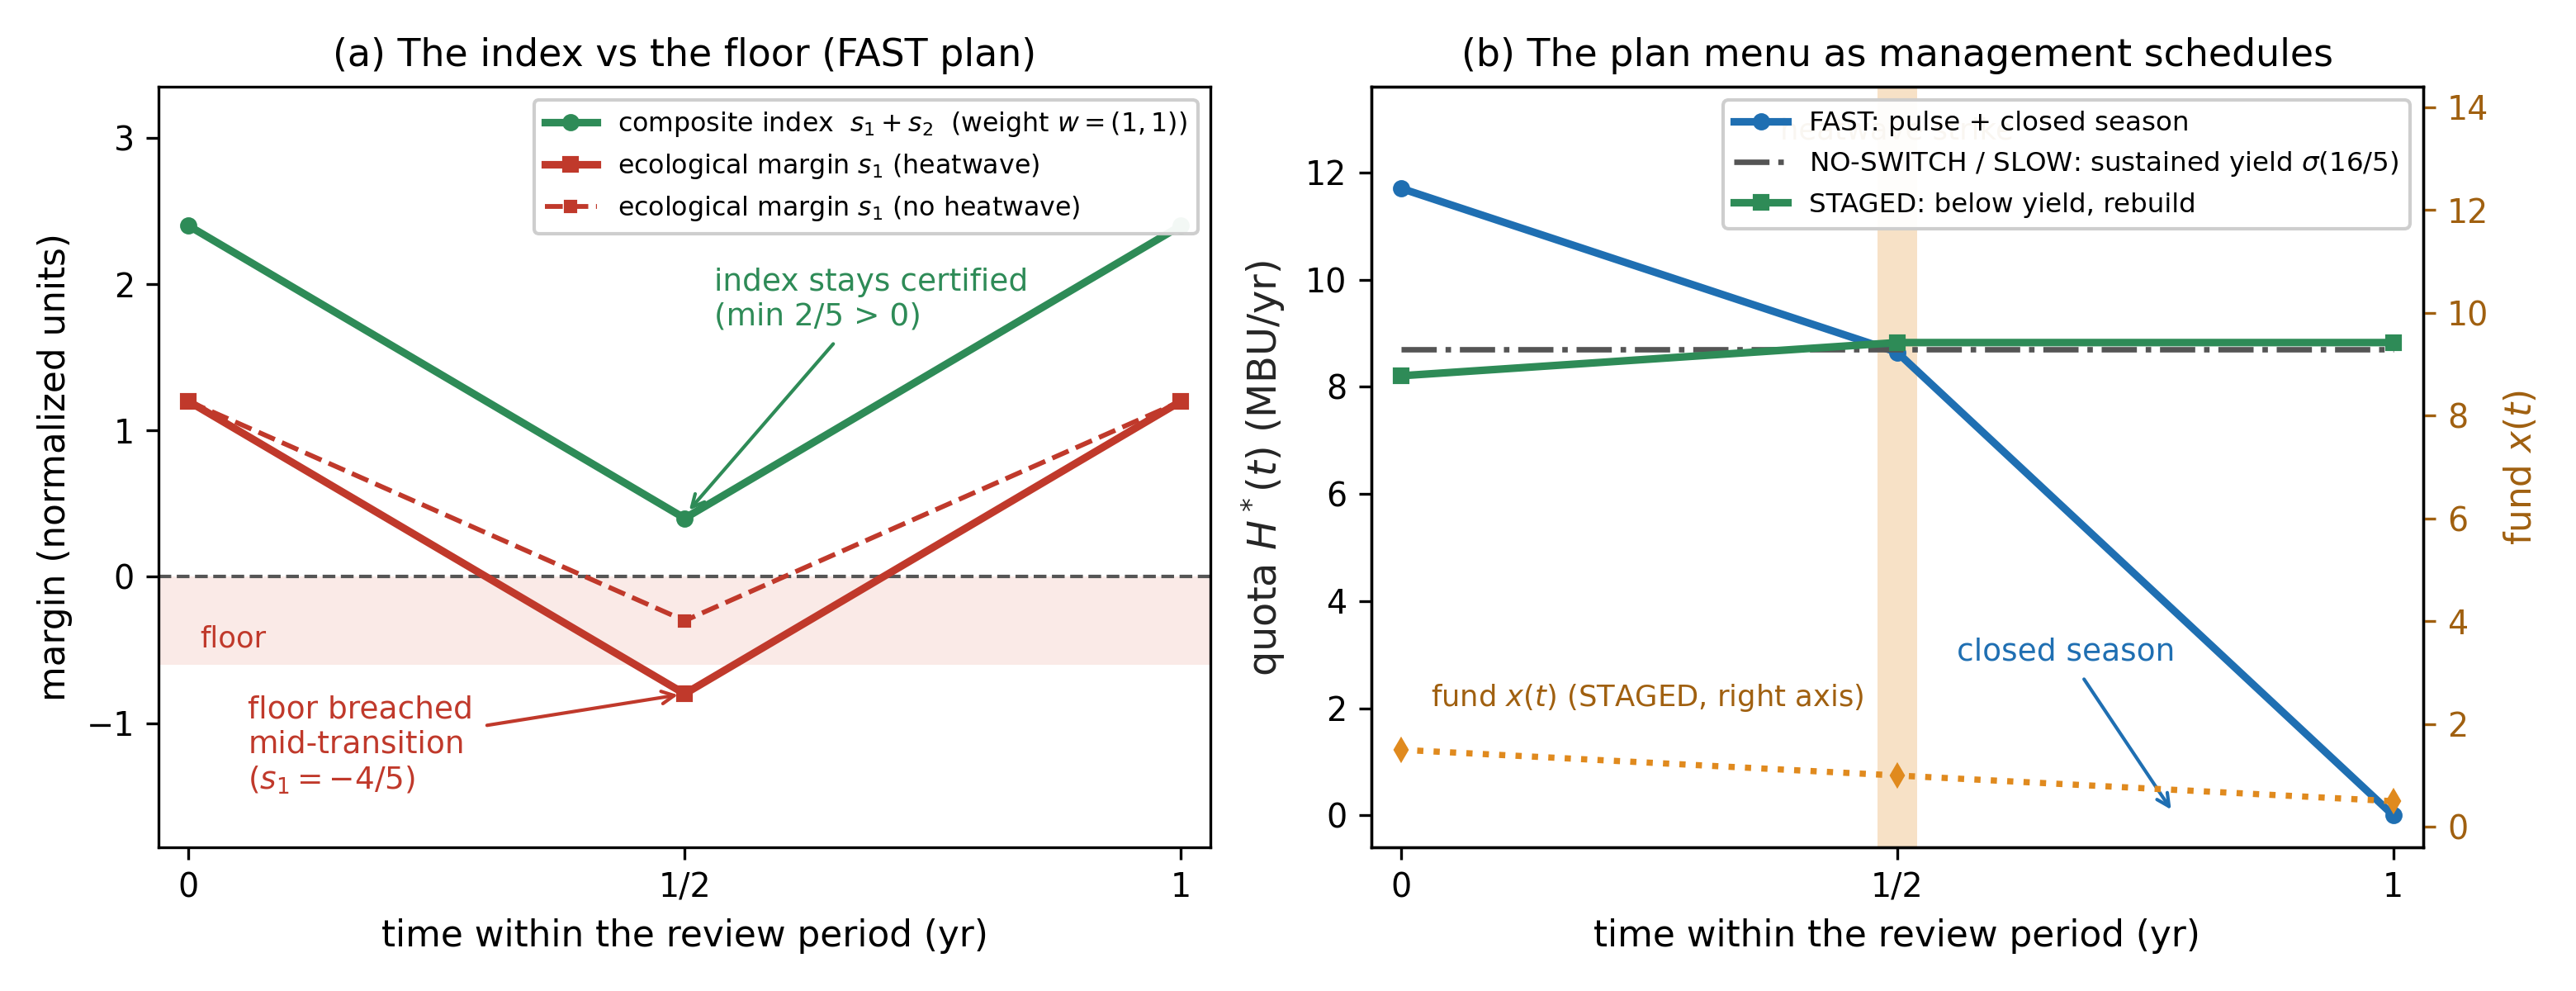
\includegraphics[width=0.96\linewidth]{fig_benchmark.png}
\caption{The witness datum read as an illustrative resource transition. (a) The constructed normalized index $s_1+s_2$ remains positive while the biomass margin breaches its floor. (b) The quota schedule is plotted in model biomass units per year (MBU/yr); the fund coordinate is normalized and carries no currency unit. The piecewise-linear tube and the nonlinear logistic recovery have different endpoint semantics, as detailed above and in SI~S5. All curves are schematic summaries of the declared datum, not empirical trajectories.}
\label{fig:benchmark}
\end{figure}

\section{Related work, and what is claimed as new}\label{sec:related}

The result combines familiar ingredients, so its scope matters. The full-cone identity and the elementary quantifier inclusion are not claimed as new. The contribution is a finite-menu transition-certification construction, with explicit assumptions on the tube and scalarization, and a bounded account of how its verdict changes under selected control and disturbance extensions.

\subsection{Scalarization and finite-menu geometry}

Weighted-sum scalarization recovers supported outcomes of multi-objective problems and can miss unsupported points on a nonconvex frontier; alternative scalarizations address that limitation \citep{Koski1985,AthanPapalambros1996,DasDennis1997,Miettinen1999,Ehrgott2005,MessacMattson2002}. Theorem~\ref{thm:menu} has related convex geometry, but its exact statement is a margin-first acceptance result: the required-margin vector is formed first and the scalarized requirement is assumed to be $w\cdot d_a$. It compares the up-closed convex hull of a finite menu with the union of the menu's orthants. This is not a new scalarization theorem, nor does it establish that every exact-tube scalarization has that form; Lemma~\ref{lem:sync} states when the two path orders agree.

The quantifier gap itself can be static. For example, the two alternative margin vectors $(-4/5,6/5)$ and $(6/5,-4/5)$ are not componentwise nonnegative, yet every nonzero nonnegative weight has at least one nonnegative alternative. In this paper, paths and disturbances specify how such margins arise and add transition-specific questions about transient breaches, terminal conditions, and implementable controls. They are an application setting, not a premise that makes the quantifier mechanism inherently dynamic. The relevant distinction from Pareto-front analysis is the decision object: acceptance of a state under a menu and a rule, rather than recovery of a particular outcome by a weighted-sum optimizer. The convex geometry is shared; the questions are not identical.

\subsection{Adjustable robustness, randomization, and physical blending}

The order $\exists a\,\forall w$ versus $\forall w\,\exists a_w$ resembles the here-and-now/wait-and-see distinction in adjustable robust optimization \citep{BenTal2004,BenTal2009}. The analogy is limited: here $w$ is an assessment weighting, not a realized uncertainty, and the result is a feasibility comparison, not a theorem that reverses the usual ordering of static and adjustable policy classes. On a common model and admissible-policy class, allowing adaptation includes the static policies; comparing a fractional physical control with a compulsory sequence of complete excursions compares different control extensions.

Fractional blending in Theorem~\ref{thm:blend} changes the physical control by allocating the primitive flows fractionally; it is not a lottery over primitive plans. In the shared-shock example at the canonical point, the best primitive worst margin is $-4/5$, while the balanced blend has worst margin $-1/20$: blending strictly improves this maximin margin but does not restore feasibility. We therefore describe the result as \emph{failure of feasibility restoration} at that point, not as randomization-proofness. Randomized decisions and their worst-case values are studied separately in robust optimization \citep{Delage2019,KrauseRoperGolovin2011,VorobeychikLi2014,Sinha2018,Sessa2020}.

Nor is the blend-versus-sequencing comparison a counterexample to Kuhn's realization-equivalence theorem. Under its hypotheses, mixed and behavioral strategies induce the same distribution over paths; equal path laws preserve probabilities of measurable safety events and distributional worst-case criteria. A deterministic fractional control instead produces a different physical path. The complete-excursion proposition below is conditional on its specified union-of-tubes control class. Under a distinct natural derivative implementation, a three-switch schedule can keep both canonical margins positive; this is not a counterexample to that conditional proposition, but it rules out a broad claim that all finite-rate switching fails. Any literal mixed-strategy interpretation would require a separate payoff, information structure, and disturbance model. Main and Randour study finite-memory strategy restrictions, but this manuscript does not establish that its control problem is an instance of their automaton model \citep{Kuhn1953,MainRandour2024}.

\subsection{Weak and strong sustainability}

The distinction formalized here is related to the weak-sustainability treatment of substitution among forms of capital and the strong-sustainability treatment of selected critical stocks as separately binding \citep{PearceAtkinson1993,Beckerman1994,Daly1995,Ayres2001,Neumayer2013,DietzNeumayer2007}. Both literatures include formal and empirical work; we do not characterize the wider debate as merely verbal, and we do not rank the doctrines. The operators idealize one transition-certification rule under each reading. The result establishes that these particular rules can disagree on a declared menu and disturbance class, not that any boundary or criterion ought normatively to be noncompensatory.

\subsection{Bounded contribution}

The paper's contribution is a source-checkable construction with four layers. First, the full-cone identity locates the gap in plan selection rather than loss of information at a fixed trajectory. Second, the finite-menu theorem gives the convex-margin description under its explicit margin-first hypothesis, and a rational witness realizes a nonempty transition-certification gap with an exact reserve threshold. Third, the paper analyzes a closed fractional-flow extension and several separately declared disturbance classes; these results are conditional on their respective control and shock models, not on a general equivalence between blending and randomization. Fourth, the CES ladder gives exact diagonal comparisons under the stated collapse convention and normalization; it does not identify a calibrated fishery index. The Northern-cod comparison is a historical dimensional anchor only.

We therefore claim neither priority for the quantifier-order observation, the standard convex-hull separation, nor the general usefulness of randomization. The claim is the explicit, reproducible scope of this particular transition-assessment construction and the boundaries of the conclusions that follow from it.

\section{Discussion}\label{sec:discussion}

\subsection{What the separation is, and what it is not}\label{sec:scope}

The scalarized operators $\{E_w\}_{w\in\Wp}$ formalise one compensatory certification rule: a plan is assessed through a weighted aggregate of the declared normalized margins, with the stated disturbances respected. The weak-sustainability literature is broader than this operator, encompassing aggregate wealth, nondeclining comprehensive consumption, shadow prices and intertemporal investment conditions \citep{Solow1974,Asheim1994,DasguptaMaler2000,Neumayer2013}. Strong-sustainability frameworks are also broader than the rule that every coordinate remain nonnegative at every instant; critical-natural-capital and safe-operating-space approaches include thresholds, irreversibility and resilience \citep{Ekins2003,Rockstrom2009,Raworth2012,DoyenGajardo2020}. The two operators are therefore idealized certification protocols, not definitions of the full doctrines.

The established gap is one of plan selection: every weighting may license some plan even though no single plan satisfies all typed floors. The quantifier order has an information interpretation only if the plan can actually be chosen after the assessment weight is known; the mathematical result itself does not assume such information or describe auditor behavior. The same mechanism can occur for static alternative vectors. In the present application, paths and disturbances add questions about transient breaches, terminal conditions, and which control extensions are implementable. The finite-menu theorem's convex geometry is a menu-selection result under margin-first scalarization; it is not evidence that the mechanism is inherently dynamic.

The rational witness is relative to its four-plan menu and declared disturbance class. A larger or differently implemented menu can shrink the gap. The reserve is deliberately excluded from the aggregate, so adding it to a real indicator could change the result. The action-indexed blend closes the gap only under the stated linear-flow assumption; the shared-shock blend improves the worst margin at the canonical point from $-4/5$ to $-1/20$ but remains infeasible. The complete-excursion result is conditional on a union-of-full-tubes policy class, while a distinct three-switch no-shock schedule is safe at the canonical margins. No general claim about finite-rate switching follows. The coupled-shock results are reading- and depth-conditional (SI~S4). Finally, all formal results concern finite-horizon exact-tube data; infinite horizons, stochastic constraints, partial observation and endogenous event times are outside the main model.

\subsection{Acceptance semantics in multi-criteria decision aiding}\label{sec:mcda}

The protocols in Table~\ref{tab:protocols} are sorting rules: they specify when a transition is classified as accepted or rejected, the sorting problem of decision aiding \citep{Roy1996,Vincke1992}. The licensing thresholds of Theorem~\ref{thm:witness} are weight-sensitivity intervals, analogous to sensitivity analyses for composite-indicator rankings \citep{Nardo2008,Becker2017}, but the object is which plan is licensed rather than a rank. Existing MCDA work analyzes compensability and outranking at fixed profiles \citep{Cinelli2014,Schar2025}; here the fixed-profile full-cone result is lossless (Lemma~\ref{lem:cone}), and the additional gap arises when acceptance is quantified over a finite menu.

The here-and-now/wait-and-see distinction in adjustable robust optimization is a useful analogy for common-plan versus weight-adaptive acceptance \citep{BenTal2004}. It is not a literal uncertainty model: the weight is an assessment parameter, and the result does not reverse the usual set inclusion between static and adaptive policy classes on a common model. The companion biocapacity study and obstruction-calculus paper address related applications and substitution certificates \citep{Abaee2026ecomod,Abaee2026obs}; they are not premises of the present proofs.

\subsection{Design tests for composite indicators}\label{sec:design}

For indicator developers, the results suggest four checks. Each follows from a stated theorem and applies only within its declared model.
\begin{enumerate}[leftmargin=2em]
\item \textbf{Fixed-profile losslessness.} Does the declared weight family detect every component violation on a fixed trajectory? The full nonnegative cone does (Lemma~\ref{lem:cone}); a restricted nonempty family requires its own characterization (Proposition~\ref{prop:monotone}).
\item \textbf{Protocol quantifiers.} Does certification require one plan to work for every weighting, or permit plan reselection by weight? If the latter, report the plan ranges and the menu-relative gap.
\item \textbf{Path and endpoint checks.} Is the assessment evaluated on the full tube or only at sampled endpoints? The witness's fast plan is typed-endpoint-admissible even where its tube breaches a floor, so endpoint-only review can miss a transient violation.
\item \textbf{Menu and control implementation.} Is the menu exhaustive, and can fractional controls actually be implemented? The convex-hull theorem is margin-first; the physical blend requires a separately verified control law. Declare the disturbance class and do not infer feasibility from an abstract convex combination alone.
\end{enumerate}

Where floors are separately binding, reporting per-floor path minima, the reserve and the acceptance protocol allows this class of discrepancy to be reconstructed. Floors alone do not determine whether a reserve-financed rescue is available, and an aggregate without path and reserve data does not recover the typed verdict on the witness family. This is a conditional design recommendation, not a universal prescription for sustainability assessment. A ten-point checklist, a minimum report and empirical-data requirements appear in SI~S6.

\subsection{Limitations}\label{sec:limitations}

\begin{enumerate}[label=(\roman*),leftmargin=2em]
\item The separation is an existence result on one declared finite menu; it does not estimate the size or frequency of a gap in applications.
\item The finite-menu convex-hull theorem assumes margin-first requirements $m_a(w)=w\cdot d_a$. The synchronization lemma states when that formula agrees with an exact-tube scalarization.
\item A physically implemented convexified control is an additional model and institutional assumption. Without it, convexification in required-margin space is only geometric.
\item The hold-prefix persistence result is proved for its specified extension. A separate repair-stage example shows one erasure mechanism; it does not imply that arbitrary continuations, coincident endpoint sets, or action coupling erase pathwise gaps.
\item The biomass illustration is synthetic. Its optional mapping to the historical DFO limit implies very large model capacities, and its nonlinear recovery does not return to the abstract successor without additional terminal control. The income-margin paths are stipulated rather than generated from an economic model.
\item CES results use the explicit collapse convention and the normalization $\lambda_i=1+s_i$. The diagonal thresholds are analytic; the off-diagonal formula is stated separately, while no global fixed-sum stationary-point or phase theorem is claimed. The common-shock statements apply only to the specified decomposition.
\item The finite rational verifiers check enumerated instances, not continua. The Lean source formalizes selected components and does not cover the full real-exponent, continuity, or topological steps; version and artifact limitations are detailed in SI~S7.
\item Novelty statements are bounded by the literature comparisons in Section~\ref{sec:related}; no claim is made that composite-index or sustainability scholarship lacks formal analysis.
\end{enumerate}

\section{Conclusions}\label{sec:conclusions}

At a fixed trajectory, aggregation over the full nonnegative cone is lossless. A separation can nevertheless arise when the assessment rule permits each weight to select a different plan. For finite menus under the explicit margin-first hypothesis, the accepted-set gap is the part of the up-closed convex hull of required margins not covered by any single plan's orthant. A rational transition witness realizes a nonempty gap and an exact reserve threshold. This is a menu-selection result that can be static; pathwise tubes and disturbances specify its application to transition certification.

Under the witness's linear-flow assumption, a fractional physical blend closes the action-indexed gap. A complete-excursion concatenation preserves primitive floor violations only under its stipulated union-of-tubes semantics, and another finite-switch extension can be safe. Under the specified shared-shock class, the gap survives an exact $1/2$-cut and the balanced blend improves but does not restore feasibility at the canonical point. On the witness-defined diagonal, every positive-elasticity CES member falsely certifies an exact interval under the stated collapse convention, whereas the Leontief limit reproduces typed acceptance over the full weight family. These are model-specific statements, not general claims about randomization, all switching policies, or real fishery dynamics.

For transition reporting, the practical conclusion is to declare the menu, the disturbance class, the normalized margin scales, the plan-selection rule, the path minima, the terminal treatment, and any resource needed for rescue. An aggregate can remain positive while a typed floor is breached, but the example does not show that every composite index is unsound or that a particular policy doctrine is normatively required. The benchmark is a transparent dimensional illustration anchored to a historical DFO value, not a fitted or predictive cod model.

\appendix

\section{Proofs of the general results}\label{app:general}

\begin{proof}[Proof of Lemma~\ref{lem:quant}]
If $a\in\bigcap_\lambda E_\lambda(z)$ then each $E_\lambda(z)$ is nonempty, so $z$ lies in the right-hand set. The inclusion fails at $z$ precisely when each $E_\lambda(z)$ is nonempty but $\bigcap_\lambda E_\lambda(z)=\varnothing$, i.e.\ when no common selector exists, which is the stated equality condition.
\end{proof}

\begin{proof}[Proof of Lemma~\ref{lem:cone}]
($\Rightarrow$) $w\ge0$, $w\ne0$, $v\ge0$ give $w\cdot v=\sum_iw_iv_i\ge0$. ($\Leftarrow$) If $v_k<0$, take $w=e_k\in\Wp$ (the $k$-th standard basis vector): $w\cdot v=v_k<0$.
\end{proof}

\begin{proof}[Proof of Proposition~\ref{prop:hierarchy}]
(i) Let $a\in\Etyp(z)$. For every $d$, $\Tube(a,d)\subseteq S=S^{\mathrm{phys}}\cap\{s\ge0\}$; by Lemma~\ref{lem:cone} every tube point satisfies $w\cdot s\ge0$ for every $w\in\Wp$, and likewise every successor lies in $G^w$, so $a\in E_w(z)$. The remaining inclusions follow from $S^w\subseteq S^{\mathrm{phys}}$, $G^w\subseteq G^{\mathrm{phys}}$ and $\End(a,d)\subseteq\Tube(a,d)$.
(ii) The inclusion $\subseteq$ is (i) intersected over $w$. Conversely let $a\in\bigcap_{w\in\Wp}E_w(z)$. For every $d$ and every tube point $p$, $w\cdot s(p)\ge0$ for every $w\in\Wp$, so $s(p)\ge0$ componentwise by Lemma~\ref{lem:cone}; hence $\Tube(a,d)\subseteq S$, and the same argument with $\Succ$ gives $\Succ(a,d)\subseteq G$. Thus $a\in\Etyp(z)$.
\end{proof}

\begin{proof}[Proof of Proposition~\ref{prop:monotone}]
The proposition assumes $W\ne\varnothing$. By Proposition~\ref{prop:hierarchy}(i), $E_w(z)\subseteq\Ephys(z)$ for every $w$, so $\mathcal V_w\subseteq\Vphys$ and a nonempty intersection over $W$ remains a subset of $\Vphys$. If $z\in\Vtyp$, Proposition~\ref{prop:hierarchy}(ii) gives $a\in\bigcap_{w\in\Wp}E_w(z)\subseteq\bigcap_{w\in W}E_w(z)$, so $z\in\mathcal V_W$. Monotonicity follows because intersecting over a larger family can only shrink the intersection.
\end{proof}

\begin{proof}[Proof of Theorem~\ref{thm:menu}]
The margin-first hypothesis identifies the scalarized test with $w\cdot d_a\le w\cdot s$ for each plan; without it, the following convex-hull identity need not describe the exact-tube operator. (i) is the margin test restated. For (ii), if $s=d+v$ with $d\in\conv(\mathcal D)$ and $v\ge0$, then for every $w\ge0$, $w\cdot s\ge w\cdot d\ge\min_aw\cdot d_a$, so the scalarized test holds. Conversely suppose $s\notin\conv(\mathcal D)+\Rp$. This set is closed and convex (a compact polytope plus a closed cone), so strict separation gives $w\ne0$ with $w\cdot s<w\cdot d+w\cdot v$ for every $d\in\conv(\mathcal D)$ and every $v\ge0$. Strict separation supplies $w\ne0$. If some coordinate $w_i<0$, choose $v=t e_i$ and let $t\to\infty$; for any fixed $d\in\conv(\mathcal D)$ the right-hand side $w\cdot d+t w_i$ tends to $-\infty$, contradicting the separating inequality. Thus $w\ge0$, so $w\in\Rp\setminus\{0\}$. Taking $v=0$ gives $w\cdot s<\min_{d\in\conv(\mathcal D)}w\cdot d=\min_aw\cdot d_a$, so the scalarized test fails at $w$. The gap formula is (ii) minus (i); if $\mathcal D$ is replaced by $\conv(\mathcal D)$ the union in (i) becomes $\conv(\mathcal D)+\Rp$ and the gap is empty.
\end{proof}

\section{Proofs for the witness datum}\label{app:witness}

\begin{proof}[Proof of Theorem~\ref{thm:witness}]
\textbf{(1)} Typed admissibility requires the worst-case tube in $S_0$ and the successor in $G$. \act{no-switch} never reaches $G$ (its successor retains $q=0$). For \act{fast} the worst-case $s_1$-tube is $[s_1-2,s_1]$, safe iff $s_1\ge2$; its successor $(1,x,s+e)\in G$ given $x\ge0$. Symmetrically \act{slow} is typed-admissible iff $s_2\ge2$. For \act{staged} the floors grow and the successor lies in $G$; the binding constraint is the $x$-tube $[x-1,x]$, safe iff $x\ge1$. Hence $\Vtyp=\{x\ge1\}\cup\{s_1\ge2\}\cup\{s_2\ge2\}$.

\textbf{(2)} Fix $w=(w_1,w_2)\in\Wp$. \act{no-switch} misses $G^w$. \act{fast} is $w$-admissible iff its worst-case aggregate stays nonnegative, $w_1(s_1-2)+w_2s_2\ge0$, i.e.\ $w_1s_1+w_2s_2\ge2w_1$; symmetrically \act{slow} iff $w_1s_1+w_2s_2\ge2w_2$; \act{staged} iff $x\ge1$, since $w\cdot s\ge0$ holds automatically along its tube. Hence $z\in\mathcal V_w$ whenever $x\ge1$; if $x<1$, $z\in\mathcal V_w$ iff one of the two inequalities holds. If $x\ge1$ then $z\in\Vweak$. If $x<1$ and, say, $s_1\ge2$, \act{fast} is typed-admissible by (1), hence $w$-admissible for every $w$, so $z\in\Vweak$. It remains to treat $x<1$, $s_1<2$, $s_2<2$. For $w_1>0$ write $r=w_2/w_1$: \act{fast} is licensed iff $s_1+rs_2\ge2$, i.e.\ $r\ge(2-s_1)/s_2=\rho_1$ (for $s_2>0$; when $s_2=0$ the condition is $s_1\ge2$, excluded), and \act{slow} iff $s_1+rs_2\ge2r$, i.e.\ $r\le s_1/(2-s_2)=\rho_2$. At $w_1=0$ ($r\to\infty$) \act{fast} is licensed provided $s_2\ge0$ while \act{slow} is rejected on $s_2<2$; at $w_2=0$ ($r=0$) symmetrically. Therefore $z\in\mathcal V_w$ for every $w$ iff $\{r\ge\rho_1\}\cup\{r\le\rho_2\}=[0,\infty]$, i.e.\ iff $\rho_2\ge\rho_1$, and
\[
\frac{s_1}{2-s_2}\ge\frac{2-s_1}{s_2}\iff s_1s_2\ge(2-s_1)(2-s_2)\iff s_1+s_2\ge2,
\]
both denominators being positive. Assembling the cases, and noting $\{s_1\ge2\}\cup\{s_2\ge2\}\subseteq\{s_1+s_2\ge2\}$ under nonnegativity, $\Vweak=\{x\ge1\}\cup\{s_1+s_2\ge2\}$.

\textbf{(3)} The physical operators constrain only $x\ge0$ (with $q=1$ at the destination). \act{fast} and \act{slow} have tubes in $S^{\mathrm{phys}}$ and successors in $G^{\mathrm{phys}}$ for every $z\in X_0$ (their dips affect only $s$), so $\Vphys=X_0$; their endpoint values likewise, so $\Vend=X_0$.

\textbf{(4)} By (1)--(2), $\FP=[\{x\ge1\}\cup\{s_1+s_2\ge2\}]\setminus[\{x\ge1\}\cup\{s_1\ge2\}\cup\{s_2\ge2\}]=\{x<1,\ s_1<2,\ s_2<2,\ s_1+s_2\ge2\}=I$, nonempty (e.g.\ $(\tfrac12,\tfrac65,\tfrac65)$) with the stated interior; $R\subseteq\{x\ge1\}\subseteq\Vtyp$.

\textbf{(5)} The first strictness is (4). The point $(\tfrac12,\tfrac1{10},\tfrac1{10})$ has $x<1$ and $s_1+s_2=\tfrac15<2$, so it is outside $\Vweak$ by (2) and inside $\Vphys$ by (3).

\textbf{(6)} The threshold characterisation was derived in (2). On $\Q$, $s_1+s_2\ge2$, so the two licensing intervals overlap and cover all weights; on the relative interior ($s_1+s_2>2$) both thresholds are finite and $r>\rho_2$ licenses \act{fast} only, $r<\rho_1$ \act{slow} only. On $I$ ($x<1$) \act{staged} is inadmissible for every $w$, so $\Etyp(z)=\bigcap_wE_w(z)=\varnothing$ by Proposition~\ref{prop:hierarchy}(ii). On $R$ ($x\ge1$) \act{staged} lies in $\Etyp(z)$ and serves every weight.

\textbf{(7)} On $R$, \act{staged}'s tube is $[x-1,x]\times\{s\to s+e\}$ with $x\ge1$, the floors grow, and the successor $(1,x-1,s+e)\in G$. On $I$ the four violations exhaust the menu: \act{fast}'s $s_1$-tube reaches $s_1-2<0$; \act{slow}'s $s_2$-tube reaches $s_2-2<0$; \act{staged}'s $x$-tube reaches $x-1<0$; \act{no-switch}'s successor misses $G$.
\end{proof}

\begin{proof}[Proof of Theorem~\ref{thm:blend}]
(i) \act{fast}'s worst-case tube has $s_1$-coordinates $[s_1-2,s_1]$ and $s_2$-coordinate $\{s_2\}$; \act{slow}'s is the mirror; both keep $x$ nonnegative. The blended tube therefore has $s_1$-coordinates $[s_1-2\delta,s_1]$, $s_2$-coordinates $[s_2-2(1-\delta),s_2]$, and nonnegative $x$. Typed admissibility requires the tube within $S_0$ and the successor in $G$; the tube condition is exactly $\delta\le s_1/2$ and $\delta\ge1-s_2/2$, and the blended successor is the mixture of two equal successors $(1,x,s+e)\in G$. The window is nonempty iff $1-s_2/2\le s_1/2$, i.e.\ $s_1+s_2\ge2$; on $\Q$ it lies in $(0,1)$ automatically, and at equality it is the singleton $\delta=s_1/2$, feasible because $S_0$ is closed.
(ii) If $s_1+s_2\ge2$, (i) supplies a typed-admissible blend for every $x\ge0$; if $s_1+s_2<2$ no blend is typed-admissible, and the deterministic menu contributes $\Vtyp\subseteq\{x\ge1\}\cup\{s_1+s_2\ge2\}$. Hence the augmented typed set is $\{x\ge1\}\cup\{s_1+s_2\ge2\}=\Vweak$ by Theorem~\ref{thm:witness}(2), and nothing beyond.
(iii) Immediate from the window's dependence on $(s_1,s_2)$ alone and from typed admissibility implying $w$-admissibility for every weight.
\end{proof}

\begin{proof}[Proof of Proposition~\ref{prop:timeshare}]
By the proposition's defining control-class assumption, any policy using both primitives visits the union of their complete worst-case tubes. The \act{fast} tube remains above the first floor exactly when $s_1-2\ge0$, and the \act{slow} tube remains above the second exactly when $s_2-2\ge0$; their other floor coordinates are constant and the physical/destination constraints are unchanged. Thus the union is typed-safe exactly when $s_1\ge2$ and $s_2\ge2$, which cannot hold on $I$.
\end{proof}

\begin{proof}[Proof of Proposition~\ref{prop:rescue}]
Only $\act{staged}_\kappa$ depends on $\kappa$, and its typed admissibility is independent of the floors: its $x$-tube is $[x+\kappa-1,x+\kappa]$, the floors are nondecreasing, and the successor $(1,x+\kappa-1,s+e)\in G$ exactly when $x+\kappa\ge1$. If $z\in\Vtyp$ some base plan is admissible at $\kappa=0$, so $\kappa^*(z)=0$. If $z\notin\Vtyp$ -- $x<1$, $s_1<2$, $s_2<2$ -- then \act{no-switch}, \act{fast} and \act{slow} all fail by Theorem~\ref{thm:witness}(1), the only admissible element of $\mathcal A_\kappa$ is $\act{staged}_\kappa$, admissible exactly for $\kappa\ge1-x$; hence $\kappa^*(z)=1-x$.
\end{proof}

\noindent The proofs of Proposition~\ref{prop:persist}, Theorem~\ref{thm:ladder} and Proposition~\ref{prop:commonshock} are given in SI~S2; the master-equation reduction behind Theorem~\ref{thm:ladder} is the averaging argument that the two principal plans' acceptance conditions are affine in the weight share and sum to a weight-independent quantity, so that the equal weight is always the binding one on the diagonal.

\section*{Declarations}
\paragraph{Availability of data and materials} The Paper06 v77 source, figures, assembled TeX, PDFs and local build/QA record are included in this local-only package; v77 has no DOI and has not been externally deposited. The Figshare v3 record \citep{Abaee2026code} contains an exact-integer grid verifier, results/report and figure materials, but its attached manuscript is Paper1 v42, not this v77 article. The SafeTransition 1.3.0 Figshare v1 deposit \citep{Abaee2026software} contains software and benchmark artifacts, not this Paper06 manuscript. The Lean source is pinned at commit \texttt{6f626ee48b2a3a59282b5df5adda76c8d5993fdc}: \href{https://github.com/MIKEAA2020/general-sustainability/blob/6f626ee48b2a3a59282b5df5adda76c8d5993fdc/lean/Formalizations/P1_AssessmentSeparation.lean}{source}. Its header excludes the general real-exponent nesting, continuity/IVT and topological steps; no Lean build was run for v77. Scripts and logs for the historically reported ladder, off-diagonal and common-shock lists were not located in the inspected DOI packages; the finite fixed-sum/tangency scan is not a global certificate and is not used as a v77 theorem. The v77 package records which checks are available and which remain non-reproducible from versioned deposits. The preceding v75 public archive is at GitHub commit \texttt{0208f8b1523446a32ef48cbfe50415fe7ec78947}: \href{https://github.com/MIKEAA2020/general-sustainability/tree/0208f8b1523446a32ef48cbfe50415fe7ec78947/companion_restorations_20261026/Paper06_v75}{Paper06 v75}; v76 and v77 remain local. The DFO 2016 value is used only as a historical dimensional comparison; no parameter is estimated, no new empirical dataset is generated or fitted, and no empirical fit, forecast or validation is claimed.
\paragraph{Competing interests} The author declares no competing interests.
\paragraph{Funding} Not applicable.
\paragraph{Author contributions} A.A.\ conceptualized the entire work, wrote, reviewed and edited the manuscript.
\paragraph{AI declaration} GLM (Z.ai), Qwen (Alibaba Cloud) and DeepSeek AI assisted with drafting and iterative review; all results, proofs and verifications were checked by the author.

\section*{Supplementary Information}
The Supplementary Information contains: S1 abbreviations and a result map; S2 proofs of persistence, repair-stage erasure, the CES ladder and the common-shock verdict; S3 diagonal CES results, the exact off-diagonal geometric criterion, and explicitly finite exploratory fixed-sum checks; S4 the coupled and replace-reading shock variants; S5 the normalized-unit biomass illustration and historical DFO scale map; S6 practitioner material; S7 verification and Lean-coverage limits; S8 literature positioning; and S9 a compactness consequence under common compact confinement. The global fixed-sum phase claim and the earlier unproved framework extensions are not part of the current v77 SI; the latter are preserved separately as a deferred research note. File: \texttt{paper06\_assessment\_separation\_v77\_supplementary} (\texttt{.tex}/\texttt{.pdf}).

\begin{thebibliography}{99}
\makeatletter\renewcommand{\@biblabel}[1]{}\makeatother

\bibitem[Abaee(2026a)]{Abaee2026obs} Abaee, A. (2026a). An obstruction calculus for viability under incomplete observation. Manuscript; Zenodo. \url{https://doi.org/10.5281/zenodo.22552616}.

\bibitem[Abaee(2026b)]{Abaee2026ecomod} Abaee, A. (2026b). \emph{A rising biocapacity total can mask ecological-capital land drawdown: a two-land model}. Companion manuscript, c10. Exact source and PDF pinned to commit \texttt{6f626ee48b2a3a59282b5df5adda76c8d5993fdc}: \href{https://github.com/MIKEAA2020/general-sustainability/blob/6f626ee48b2a3a59282b5df5adda76c8d5993fdc/agent%202%20productivity%20illusion/output_v45_ecomod_continued_10_gemini38_v4base_si_review_20261026/ecomod_continued_10.pdf}{PDF}; \href{https://github.com/MIKEAA2020/general-sustainability/blob/6f626ee48b2a3a59282b5df5adda76c8d5993fdc/agent%202%20productivity%20illusion/output_v45_ecomod_continued_10_gemini38_v4base_si_review_20261026/ecomod_continued_10.tex}{source}.

\bibitem[Abaee(2026c)]{Abaee2026cod} Abaee, A. (2026c). Does a surplus-production ladder improve forecasts of Northern cod? A scored test on NAFO 2J3KL. Zenodo. \url{https://doi.org/10.5281/zenodo.22553609}.

\bibitem[Abaee(2026d)]{Abaee2026code} Abaee, A. (2026d). Verification code and figure pipeline for ``Aggregate indices and transition safety''. Figshare, version 3. The attached manuscript is Paper1 v42, an earlier edition in the same research line, not the local Paper06 v77 manuscript. \url{https://doi.org/10.6084/m9.figshare.33764023.v3}.
\bibitem[Abaee(2026e)]{Abaee2026software} Abaee, A. (2026e). \emph{SafeTransition: exact rational certification of transition safety for sustainability assessment}. Software release 1.3.0, Figshare, version 1. \url{https://doi.org/10.6084/m9.figshare.33971389.v1}.

\bibitem[Asheim(1994)]{Asheim1994} Asheim, G.~B. (1994). Net national product as an indicator of sustainability. \emph{Scandinavian Journal of Economics}, 96(2), 257--265.

\bibitem[Athan and Papalambros(1996)]{AthanPapalambros1996} Athan, T. W., Papalambros, P. Y. (1996). A note on weighted criteria methods for compromise solutions in multi-objective optimization. \emph{Engineering Optimization}, 27(2), 155--176.

\bibitem[Aubin and Catt\'e(2002)]{AubinCatte2002} Aubin, J.-P., and Catt\'e, F. (2002). Bilateral fixed-points and algebraic properties of viability kernels and capture basins of sets. \emph{Set-Valued Analysis}, 10(4), 379--416.

\bibitem[Aubin et~al.(2011)]{Aubin2011} Aubin, J.-P., Bayen, A.~M., and Saint-Pierre, P. (2011). \emph{Viability Theory: New Directions}, 2nd ed. Birkh\"auser, Boston.

\bibitem[Aubin(1991)]{Aubin1991} Aubin, J.-P. (1991). \emph{Viability Theory}. Birkh\"auser, Boston.

\bibitem[Ayres et al.(2001)]{Ayres2001} Ayres, R. U., van den Bergh, J. C. J. M., Gowdy, J. M. (2001). Strong versus weak sustainability: economics, natural sciences, and ``consilience''. \emph{Environmental Ethics}, 23(2), 155--168.

\bibitem[Becker et~al.(2017)]{Becker2017} Becker, W., Saisana, M., Paruolo, P., and Vandecasteele, I. (2017). Weights and importance in composite indicators: Closing the gap. \emph{Ecological Indicators}, 80, 12--22.

\bibitem[Beckerman(1994)]{Beckerman1994} Beckerman, W. (1994). `Sustainable development': is it a useful concept? \emph{Environmental Values}, 3(3), 191--209.

\bibitem[Ben-Tal et~al.(2004)]{BenTal2004} Ben-Tal, A., Goryashko, A., Guslitzer, E., and Nemirovski, A. (2004). Adjustable robust solutions of uncertain linear programs. \emph{Mathematical Programming}, 99(2), 351--376.

\bibitem[Ben-Tal et al.(2009)]{BenTal2009} Ben-Tal, A., El Ghaoui, L., Nemirovski, A. (2009). \emph{Robust Optimization}. Princeton University Press.

\bibitem[Bertsimas and Goyal(2010)]{BertsimasGoyal2010} Bertsimas, D., Goyal, V. (2010). On the power of robust solutions in two-stage stochastic and adaptive optimization problems. \emph{Mathematics of Operations Research}, 35(2), 284--305.

\bibitem[Boos(2015)]{Boos2015} Boos, A. (2015). Genuine savings as an indicator for ``weak'' sustainability: Critical survey and possible ways forward in measuring weak sustainability. \emph{Sustainability}, 7(4), 4146--4163.

\bibitem[Cairns and Martinet(2014)]{CairnsMartinet2014} Cairns, R.~D., and Martinet, V. (2014). An environmental-economic measure of sustainable development. \emph{European Economic Review}, 69, 4--17.

\bibitem[Cardaliaguet(1996)]{Cardaliaguet1996} Cardaliaguet, P. (1996). A differential game with two players and one target. \emph{SIAM Journal on Control and Optimization}, 34(4), 1441--1460.

\bibitem[Cinelli et~al.(2014)]{Cinelli2014} Cinelli, M., Coles, S.~R., and Kirwan, K. (2014). Analysis of the potentials of multi criteria decision analysis methods to conduct sustainability assessment. \emph{Ecological Indicators}, 46, 138--148.

\bibitem[Daly(1990)]{Daly1990} Daly, H.~E. (1990). Toward some operational principles of sustainable development. \emph{Ecological Economics}, 2(1), 1--6.

\bibitem[Daly(1995)]{Daly1995} Daly, H. E. (1995). On Wilfred Beckerman's critique of sustainable development. \emph{Environmental Values}, 4(1), 49--55.

\bibitem[Das and Dennis(1997)]{DasDennis1997} Das, I., and Dennis, J.~E. (1997). A closer look at drawbacks of minimizing weighted sums of objectives for Pareto set generation in multicriteria optimization problems. \emph{Structural Optimization}, 14, 63--69.

\bibitem[Dasgupta and M\"aler(2000)]{DasguptaMaler2000} Dasgupta, P., and M\"aler, K.-G. (2000). Net national product, wealth, and social well-being. \emph{Environment and Development Economics}, 5(1), 69--93.

\bibitem[De Lara and Doyen(2008)]{DeLaraDoyen2008} De Lara, M., and Doyen, L. (2008). \emph{Sustainable Management of Natural Resources: Mathematical Models and Methods}. Springer, Berlin.

\bibitem[Delage et al.(2019)]{Delage2019} Delage, E., Kuhn, D., Wiesemann, W. (2019). ``Dice''-sion-making under uncertainty: when can a random decision reduce risk? \emph{Management Science}, 65(7), 3282--3301.

\bibitem[DFO(2016)]{DFO2016} DFO (2016). \emph{Stock Assessment of Northern Cod (NAFO Divs.\ 2J3KL) in 2016}. Canadian Science Advisory Secretariat, Science Advisory Report 2016/026. Fisheries and Oceans Canada, Ottawa.

\bibitem[Dietz and Neumayer(2007)]{DietzNeumayer2007} Dietz, S., Neumayer, E. (2007). Weak and strong sustainability in the SEEA: concepts and measurement. \emph{Ecological Economics}, 61(4), 617--626.

\bibitem[Doyen and Gajardo(2020)]{DoyenGajardo2020} Doyen, L., and Gajardo, P. (2020). Sustainability standards, multicriteria maximin, and viability. \emph{Natural Resource Modeling}, 33(3), e12250.

\bibitem[Doyen et~al.(2012)]{Doyen2012} Doyen, L., Th\'ebaud, O., B\'en\'e, C., Martinet, V., Gourguet, S., Bertignac, M., Fifas, S., and Blanchard, F. (2012). A stochastic viability approach to ecosystem-based fisheries management. \emph{Ecological Economics}, 75, 32--42.

\bibitem[Ehrgott(2005)]{Ehrgott2005} Ehrgott, M. (2005). \emph{Multicriteria Optimization} (2nd ed.). Springer.

\bibitem[Ekins et~al.(2003)]{Ekins2003} Ekins, P., Simon, S., Deutsch, L., Folke, C., and De Groot, R. (2003). A framework for the practical application of the concepts of critical natural capital and strong sustainability. \emph{Ecological Economics}, 44(2), 165--185.

\bibitem[Fabian et~al.(2010)]{Fabian2010} Fabian, M.~J., Henrion, R., Kruger, A.~Y., and Outrata, J.~V. (2010). Error bounds: necessary and sufficient conditions. \emph{Set-Valued and Variational Analysis}, 18(2), 121--149.

\bibitem[Fanning et~al.(2022)]{Fanning2022} Fanning, A.~L., O'Neill, D.~W., Hickel, J., and Roux, N. (2022). The social shortfall and ecological overshoot of nations. \emph{Nature Sustainability}, 5(1), 26--36.

\bibitem[Filippov(1988)]{Filippov1988} Filippov, A.~F. (1988). \emph{Differential Equations with Discontinuous Righthand Sides}. Kluwer, Dordrecht.

\bibitem[Fischer et~al.(2022)]{Fischer2022} Fischer, S.~M., Joy, M.~K., Abrahamse, W., Milfont, T.~L., and Petherick, L.~M. (2022). The use and misuse of composite environmental indices. \emph{bioRxiv}, 2022.03.15.484501. \url{https://doi.org/10.1101/2022.03.15.484501}.

\bibitem[Frankowska(1989)]{Frankowska1989} Frankowska, H. (1989). Optimal trajectories associated with a solution of contingent Hamilton--Jacobi equations. \emph{Applied Mathematics and Optimization}, 19, 291--311.

\bibitem[Gao et~al.(2023)]{Gao2023} Gao, P., Wang, Y., Wang, H., Song, C., Ye, S., and Wang, X. (2023). A Pareto front-based approach for constructing composite index of sustainability without weights: A comparative study of implementations. \emph{Ecological Indicators}, 155, 110919.

\bibitem[Hanley et~al.(1999)]{Hanley1999} Hanley, N., Moffatt, I., Faichney, R., and Wilson, M. (1999). Measuring sustainability: A time series of alternative indicators for Scotland. \emph{Ecological Economics}, 28(1), 55--73.

\bibitem[Hickel(2020)]{Hickel2020} Hickel, J. (2020). The sustainable development index: Measuring the ecological efficiency of human development in the Anthropocene. \emph{Ecological Economics}, 167, 106331.

\bibitem[Keeney and Raiffa(1976)]{KeeneyRaiffa1976} Keeney, R.~L., and Raiffa, H. (1976). \emph{Decisions with Multiple Objectives: Preferences and Value Tradeoffs}. Wiley, New York.

\bibitem[Koski(1985)]{Koski1985} Koski, J. (1985). Defectiveness of weighting method in multicriterion optimization of structures. \emph{Communications in Applied Numerical Methods}, 1(6), 333--337.

\bibitem[Krause et al.(2011)]{KrauseRoperGolovin2011} Krause, A., Roper, A., Golovin, D. (2011). Randomized sensing in adversarial environments. In \emph{Proceedings of the 22nd International Joint Conference on Artificial Intelligence (IJCAI)}, 2133--2139.

\bibitem[Kuhn(1953)]{Kuhn1953} Kuhn, H. W. (1953). Extensive games and the problem of information. In H. W. Kuhn, A. W. Tucker (Eds.), \emph{Contributions to the Theory of Games II} (Annals of Mathematics Studies 28, pp. 193--216). Princeton University Press.

\bibitem[Lade et~al.(2020)]{Lade2020} Lade, S.~J., Steffen, W., de Vries, W., Carpenter, S.~R., Donges, J.~F., Gerten, D., Hoff, H., Newbold, T., Richardson, K., and Rockstr\"om, J. (2020). Human impacts on planetary boundaries amplified by Earth system interactions. \emph{Nature Sustainability}, 3(2), 119--128.

\bibitem[Lygeros et~al.(1999)]{Lygeros1999} Lygeros, J., Tomlin, C., and Sastry, S. (1999). Controllers for reachability specifications for hybrid systems. \emph{Automatica}, 35(3), 349--370.

\bibitem[Main and Randour(2024)]{MainRandour2024} Main, J. C. A., Randour, M. (2024). Different strokes in randomised strategies: revisiting Kuhn's theorem under finite-memory assumptions. \emph{Information and Computation}, 301, 105229.

\bibitem[Martinet(2011)]{Martinet2011} Martinet, V. (2011). A characterization of sustainability with indicators. \emph{Journal of Environmental Economics and Management}, 61(2), 183--197.

\bibitem[Martinez-Alier et~al.(1998)]{MartinezAlier1998} Martinez-Alier, J., Munda, G., and O'Neill, J. (1998). Weak comparability of values as a foundation for ecological economics. \emph{Ecological Economics}, 26(3), 277--286.

\bibitem[Messac and Mattson(2002)]{MessacMattson2002} Messac, A., Mattson, C. A. (2002). Generating well-distributed sets of Pareto points for engineering design using physical programming. \emph{Optimization and Engineering}, 3(4), 431--450.

\bibitem[Miettinen(1999)]{Miettinen1999} Miettinen, K. (1999). \emph{Nonlinear Multiobjective Optimization}. Kluwer.

\bibitem[Munda and Nardo(2009)]{MundaNardo2009} Munda, G., Nardo, M. (2009). Noncompensatory/nonlinear composite indicators for ranking countries: a defensible setting. \emph{Applied Economics}, 41(12), 1513--1523.

\bibitem[Munda(2005)]{Munda2005} Munda, G. (2005). Multiple criteria decision analysis and sustainable development. In Figueira, J., Greco, S., and Ehrgott, M. (eds.), \emph{Multiple Criteria Decision Analysis: State of the Art Surveys}. Springer, New York, 953--986.

\bibitem[Nardo et~al.(2008)]{Nardo2008} Nardo, M., Saisana, M., Saltelli, A., Tarantola, S., Hoffmann, A., and Giovannini, E. (2008). \emph{Handbook on Constructing Composite Indicators: Methodology and User Guide}. OECD Publishing, Paris.

\bibitem[von Neumann(1928)]{vonNeumann1928} von Neumann, J. (1928). Zur Theorie der Gesellschaftsspiele. \emph{Mathematische Annalen}, 100, 295--320.

\bibitem[Neumayer(2013)]{Neumayer2013} Neumayer, E. (2013). \emph{Weak versus Strong Sustainability: Exploring the Limits of Two Opposing Paradigms}, 4th ed. Edward Elgar, Cheltenham.

\bibitem[O'Neill et~al.(2018)]{ONeill2018} O'Neill, D.~W., Fanning, A.~L., Lamb, W.~F., and Steinberger, J.~K. (2018). A good life for all within planetary boundaries. \emph{Nature Sustainability}, 1(2), 88--95.

\bibitem[Pearce and Atkinson(1993)]{PearceAtkinson1993} Pearce, D. W., Atkinson, G. D. (1993). Capital theory and the measurement of sustainable development: an indicator of ``weak'' sustainability. \emph{Ecological Economics}, 8(2), 103--108.

\bibitem[Raworth(2012)]{Raworth2012} Raworth, K. (2012). A safe and just space for humanity: Can we live within the doughnut? \emph{Oxfam Policy and Practice: Climate Change and Resilience}, 8(1), 1--26.

\bibitem[Rockstr\"om et~al.(2009)]{Rockstrom2009} Rockstr\"om, J., Steffen, W., Noone, K., et al. (2009). A safe operating space for humanity. \emph{Nature}, 461, 472--475.

\bibitem[Roy(1996)]{Roy1996} Roy, B. (1996). \emph{Multicriteria Methodology for Decision Aiding}. Kluwer, Dordrecht.

\bibitem[Saint-Pierre(1994)]{SaintPierre1994} Saint-Pierre, P. (1994). Approximation of the viability kernel. \emph{Applied Mathematics and Optimization}, 29, 187--209.

\bibitem[Sch\"ar et~al.(2025)]{Schar2025} Sch\"ar, S., Pohl, E., and Geldermann, J. (2025). Analysing the compensatory properties of the outranking approach PROMETHEE. \emph{Journal of Multi-Criteria Decision Analysis}, 32, e70013.

\bibitem[Schaefer(1954)]{Schaefer1954} Schaefer, M.~B. (1954). Some aspects of the dynamics of populations important to the management of commercial marine fisheries. \emph{Inter-American Tropical Tuna Commission Bulletin}, 1(2), 23--56.

\bibitem[Sessa et al.(2020)]{Sessa2020} Sessa, P. G., Bogunovic, I., Kamgarpour, M., Krause, A. (2020). Mixed strategies for robust optimization of unknown objectives. In \emph{Proceedings of the 23rd International Conference on Artificial Intelligence and Statistics (AISTATS)}, PMLR 108, 2970--2980.

\bibitem[Sinha et al.(2018)]{Sinha2018} Sinha, A., Fang, F., An, B., Kiekintveld, C., Tambe, M. (2018). Stackelberg security games: looking beyond a decade of success. In \emph{Proceedings of the 27th International Joint Conference on Artificial Intelligence (IJCAI)}, 5494--5501.

\bibitem[Sion(1958)]{Sion1958} Sion, M. (1958). On general minimax theorems. \emph{Pacific Journal of Mathematics}, 8(1), 171--176.

\bibitem[Solow(1974)]{Solow1974} Solow, R.~M. (1974). Intergenerational equity and exhaustible resources. \emph{Review of Economic Studies}, 41, 29--45.

\bibitem[Usubiaga-Lia\~no(2025)]{Usubiaga2025} Usubiaga-Lia\~no, A. (2025). Strong sustainability in the SEEA and the wider indicator debate. \emph{One Ecosystem}, 10, e141086.

\bibitem[Vincke(1992)]{Vincke1992} Vincke, P. (1992). \emph{Multicriteria Decision-Aid}. Wiley, Chichester.

\bibitem[Vorobeychik and Li(2014)]{VorobeychikLi2014} Vorobeychik, Y., Li, B. (2014). Optimal randomized classification in adversarial settings. In \emph{Proceedings of the 13th International Conference on Autonomous Agents and Multiagent Systems (AAMAS)}, 485--492.

\bibitem[Warga(1972)]{Warga1972} Warga, J. (1972). \emph{Optimal Control of Differential and Functional Equations}. Academic Press, New York.

\bibitem[Wei and Zhang(2024)]{WeiZhang2024} Wei, N., Zhang, P. (2024). Adjustability in robust linear optimization. \emph{Mathematical Programming}, 208, 581--628.

\bibitem[World Bank(2011)]{WorldBank2011} World Bank (2011). \emph{The Changing Wealth of Nations: Measuring Sustainable Development in the New Millennium}. World Bank, Washington, DC.

\end{thebibliography}

\end{document}
